\documentclass[xcolor=dvipsnames,aspectratio=1610]{beamer}

\usepackage{graphicx}
\usepackage[scale=2]{ccicons}
\usepackage{multicol}
\usepackage{enumitem}
\usepackage{xcolor}
\usepackage{algorithm, caption}
\usepackage[noend]{algpseudocode}
\usepackage[absolute,overlay]{textpos}
\usepackage{calc}
% \usepackage[texcoord,grid,gridunit=mm,gridcolor=red!10,subgridcolor=green!10]
% {eso-pic}

\setitemize{label=\usebeamerfont*{itemize item}%
  \usebeamercolor[fg]{itemize item}
  \usebeamertemplate{itemize item}}

\newcommand{\exampleheight}{1.9cm}
\newcommand{\examplewidth}{16cm}

\makeatletter
\newcommand{\algcolor}[2]{%
  \hskip-\ALG@thistlm\colorbox{#1}{\raisebox{0pt}[0.1cm][0cm]{\parbox{\dimexpr\linewidth-2\fboxsep}{\hskip\ALG@thistlm\relax #2}}}%
}
\newcommand{\algemph}[1]{\algcolor{Yellow}{#1}}
\makeatother

\usetheme[numbering=counter, progressbar=frametitle, sectionpage=none]{metropolis}
\setbeamercolor{background canvas}{bg=white}
\setbeamertemplate{caption}{\raggedright\insertcaption\par}

\title{Conflict-Free Vertex Coloring of Planar Graphs}
\date{April 15, 2017}
\author{Shawn Seymour}

\begin{document}
  \maketitle

  \begin{frame}
    \begin{figure}[h]
      \centering
      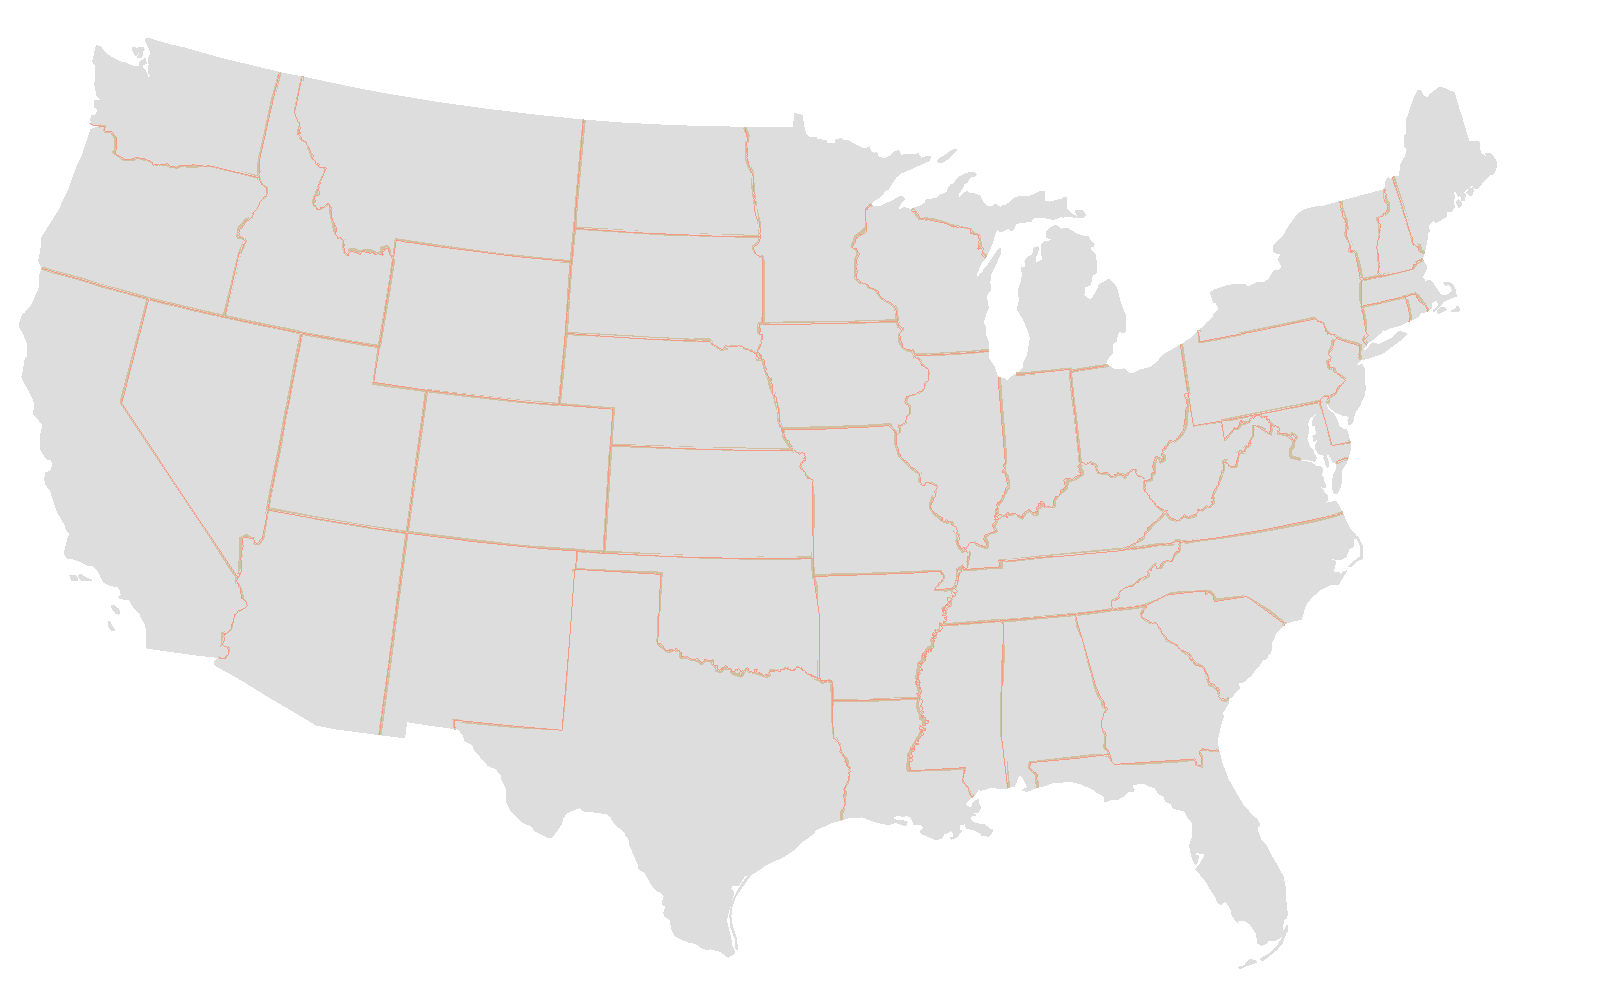
\includegraphics[width=14cm]{../figures/map-no-colors-3.pdf}
    \end{figure}
  \end{frame}

  \begin{frame}
    \begin{figure}[h]
      \centering
      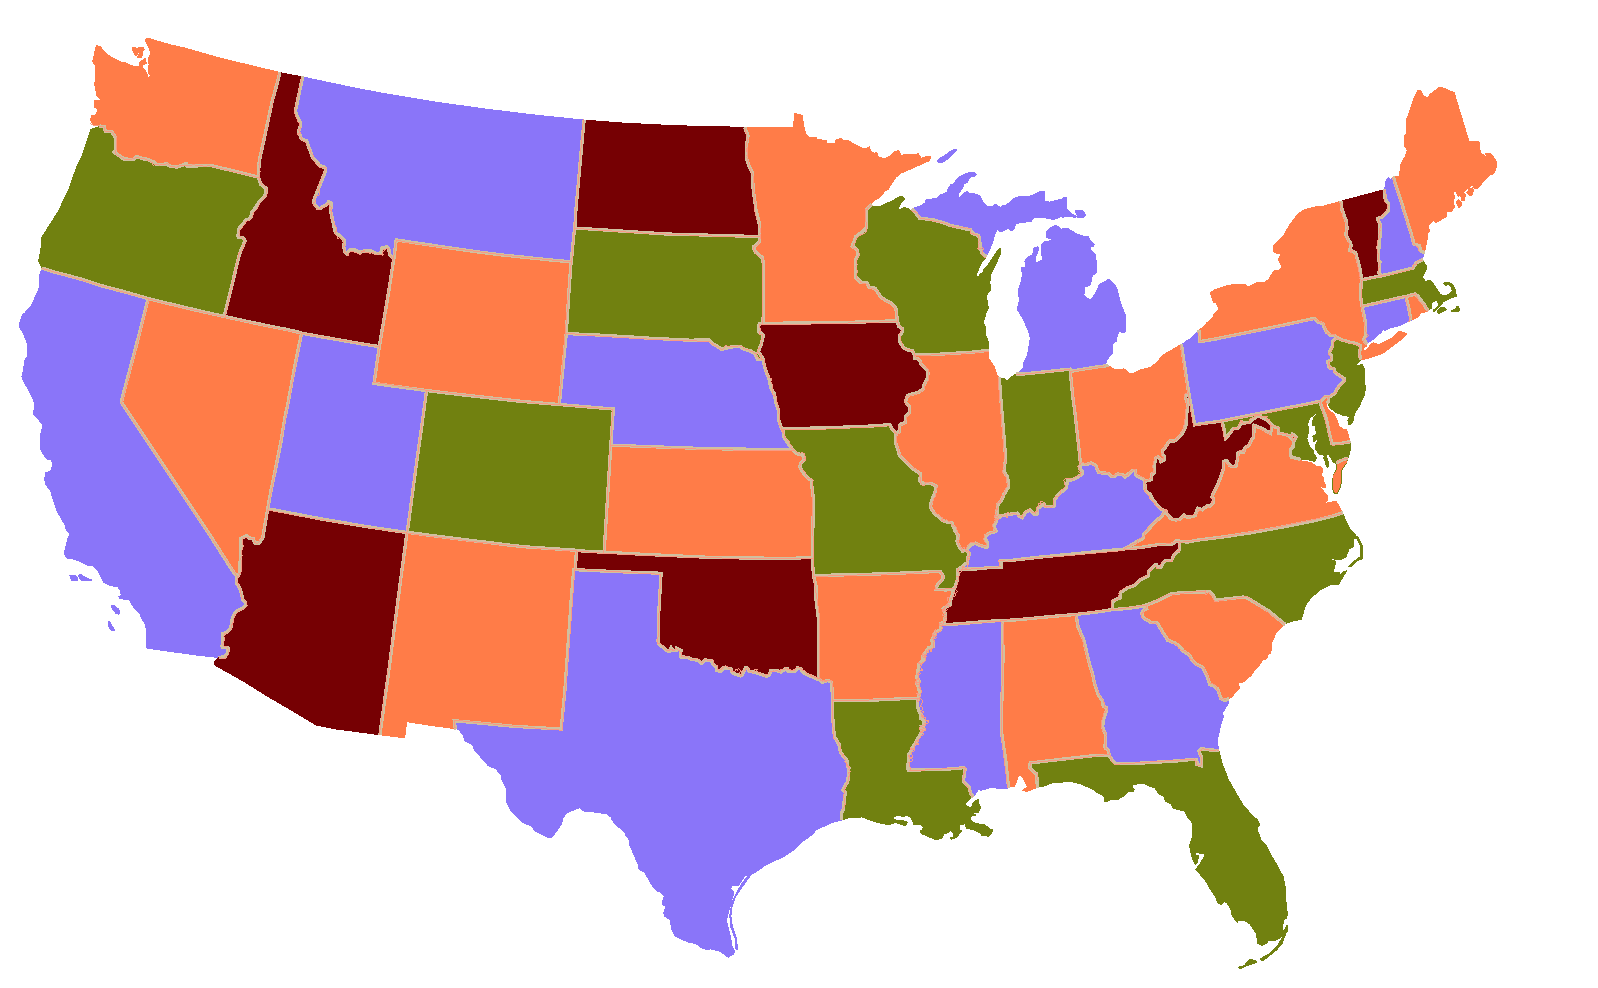
\includegraphics[width=14cm]{../figures/map-colors.pdf}
    \end{figure}
  \end{frame}

  \begin{frame}
    \frametitle{Overview}
    \begin{multicols}{2}
      \tableofcontents
    \end{multicols}
  \end{frame}

  \section{Background}

  \subsection{Graph Theory}

  \begin{frame}
    \frametitle{Graph Theory}



    \only<1-2>{
      \begin{textblock*}{\examplewidth}(0cm,\exampleheight) % {block width} (coords)
        \centering
        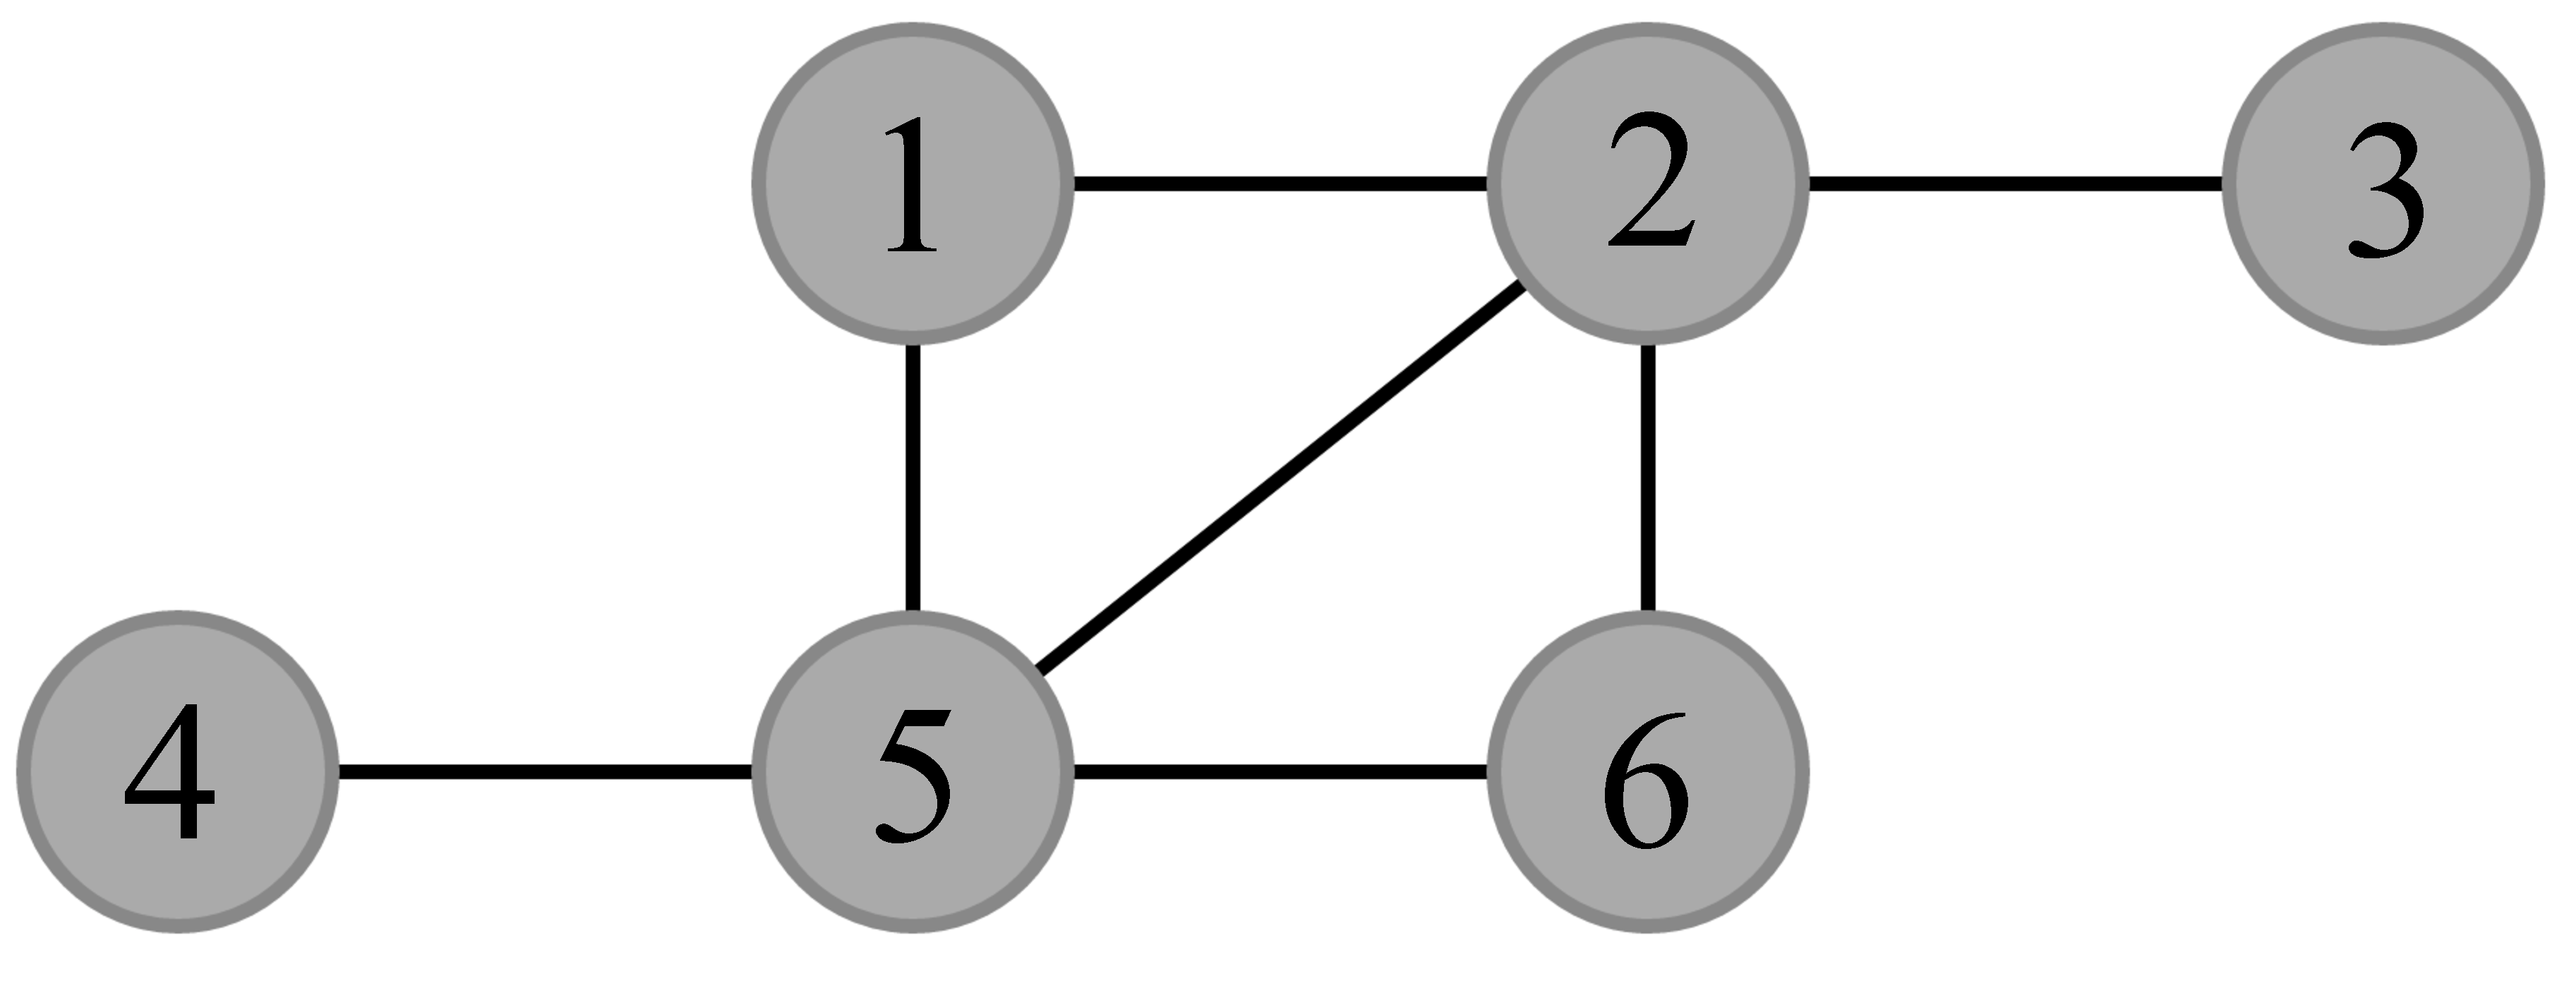
\includegraphics[width=8cm]{../figures/example.pdf}
      \end{textblock*}
    }

    \only<3> {
      \begin{textblock*}{\examplewidth}(0cm,\exampleheight) % {block width} (coords)
        \centering
        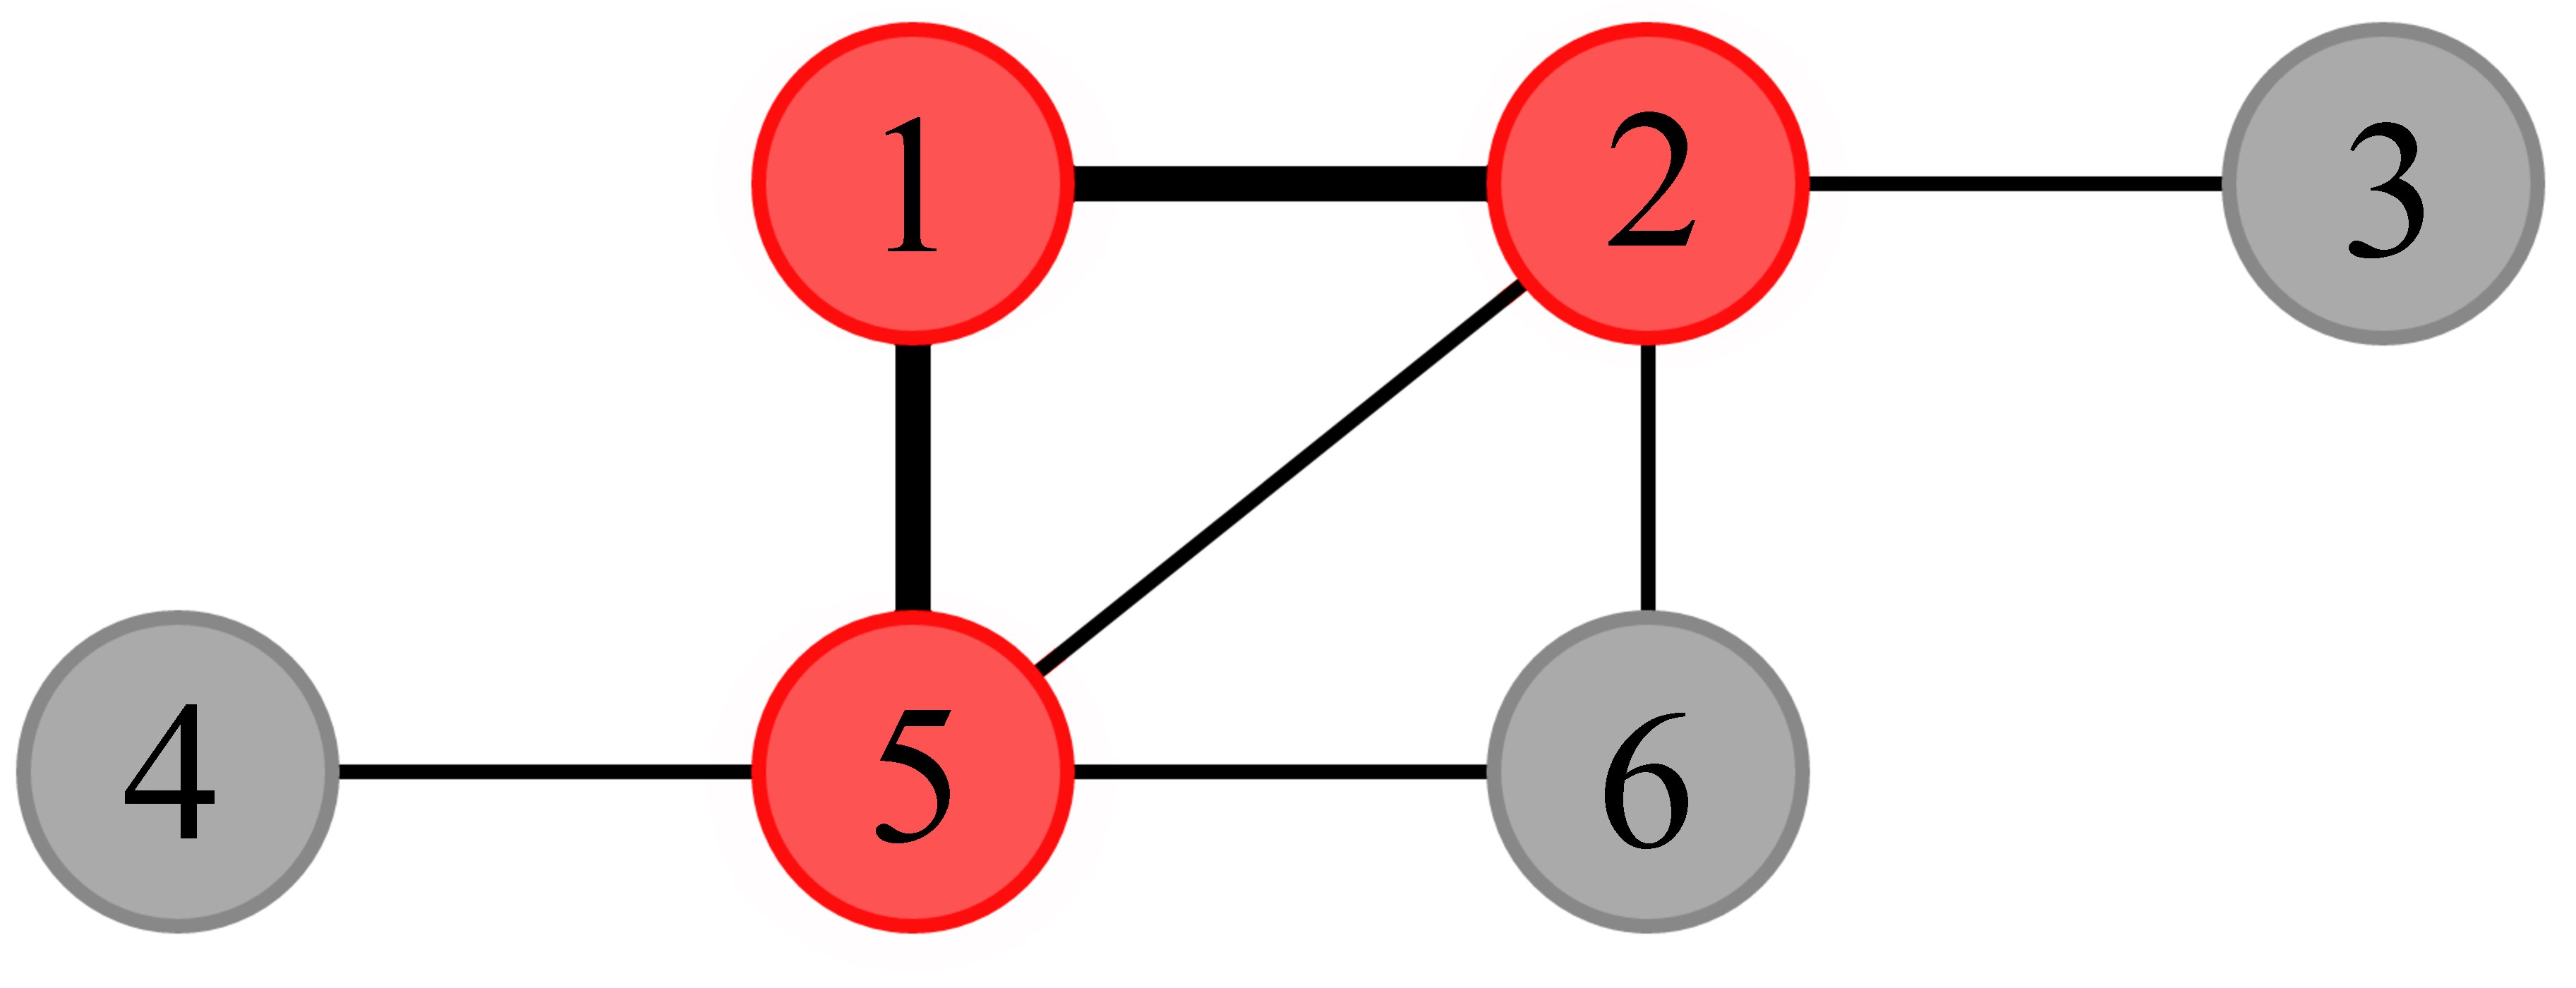
\includegraphics[width=8cm]{../figures/example-neighborhoods-1.pdf}
      \end{textblock*}
    }

    \only<4> {
      \begin{textblock*}{\examplewidth}(0cm,\exampleheight) % {block width} (coords)
        \centering
        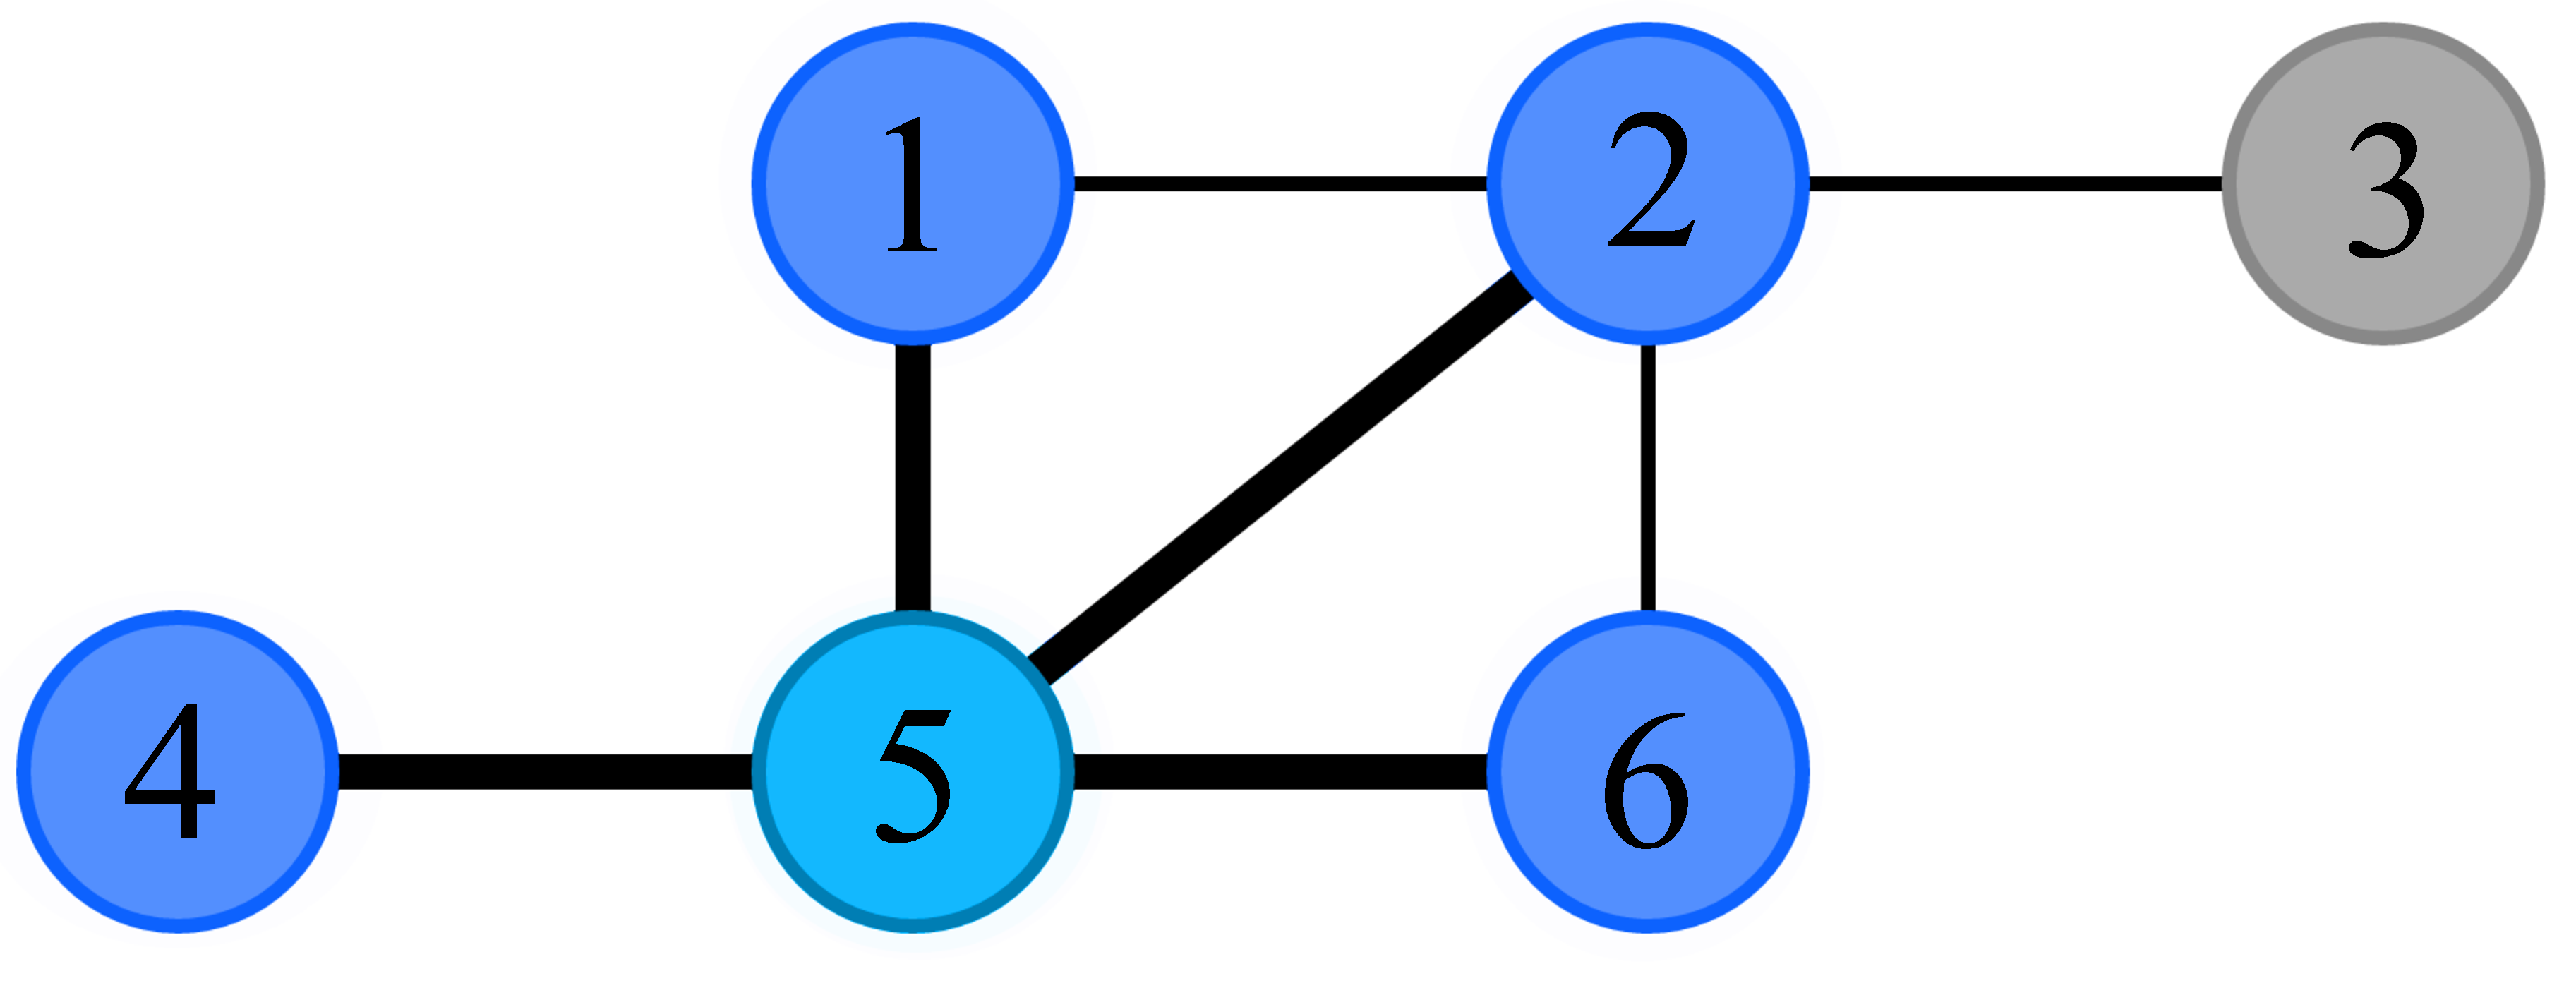
\includegraphics[width=8cm]{../figures/example-neighborhoods-2.pdf}
      \end{textblock*}
    }

    \vspace{4cm}

    \vfill

    \begin{itemize}
      \item<1-4> A \textbf{graph} is the set of vertices \emph{V} and a set of edges \emph{E}.
      \item<2-4> The \textbf{neighborhood} of a vertex $v$ is a set of all vertices adjacent to $v$ plus $v$ itself.
      \only<1-2>{\item<3> Example: The neighborhood of vertex 1: $\{1, 2, 5\}$.}
      \only<3>{\item<3> Example: The neighborhood of vertex 1: $\{1, 2, 5\}$.}
      \only<4>{\item<4> Example: The neighborhood of vertex 5: $\{1, 2, 4, 5, 6\}$.}
    \end{itemize}

  \end{frame}

  \subsection{Graph Coloring}

  \begin{frame}
    \frametitle{Vertex Coloring}

    \begin{textblock*}{\examplewidth}(0cm,\exampleheight) % {block width} (coords)
      \centering
      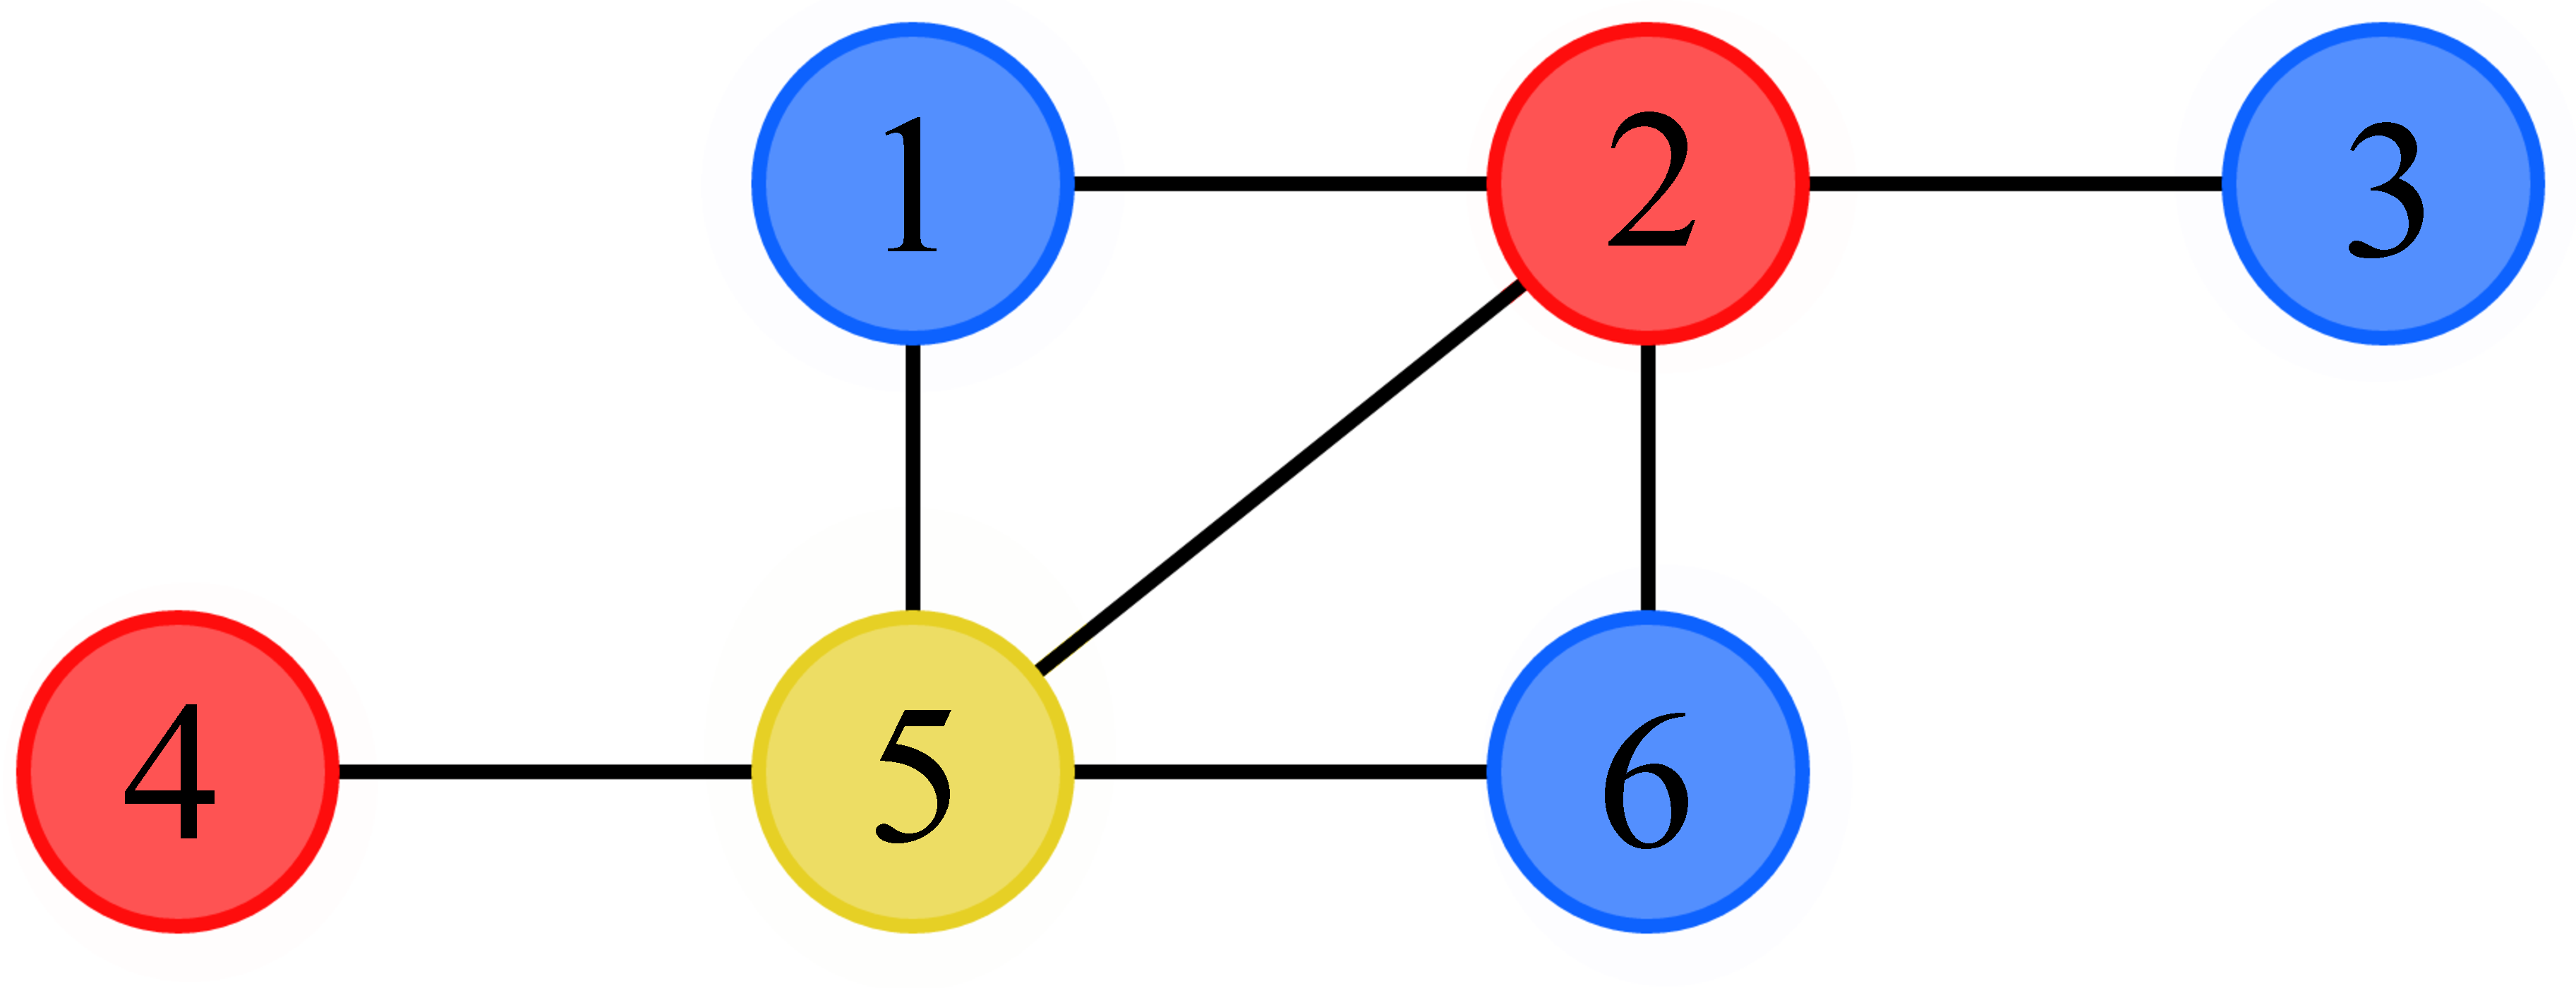
\includegraphics[width=8cm]{../figures/example-vcp.pdf}
    \end{textblock*}

    \vspace{4cm}
    \vfill

    \begin{itemize}
      \item A proper \textbf{vertex coloring} of a graph $G$ assigns colors to \emph{every} vertex such that no two adjacent vertices share the same color.
      \item The \textbf{chromatic number} of $G$ is the minimum number of colors needed to properly color $G$.
    \end{itemize}
  \end{frame}

  \begin{frame}
    \frametitle{Conflict-Free Coloring}

    \begin{textblock*}{\examplewidth}(0cm,\exampleheight) % {block width} (coords)
      \centering
      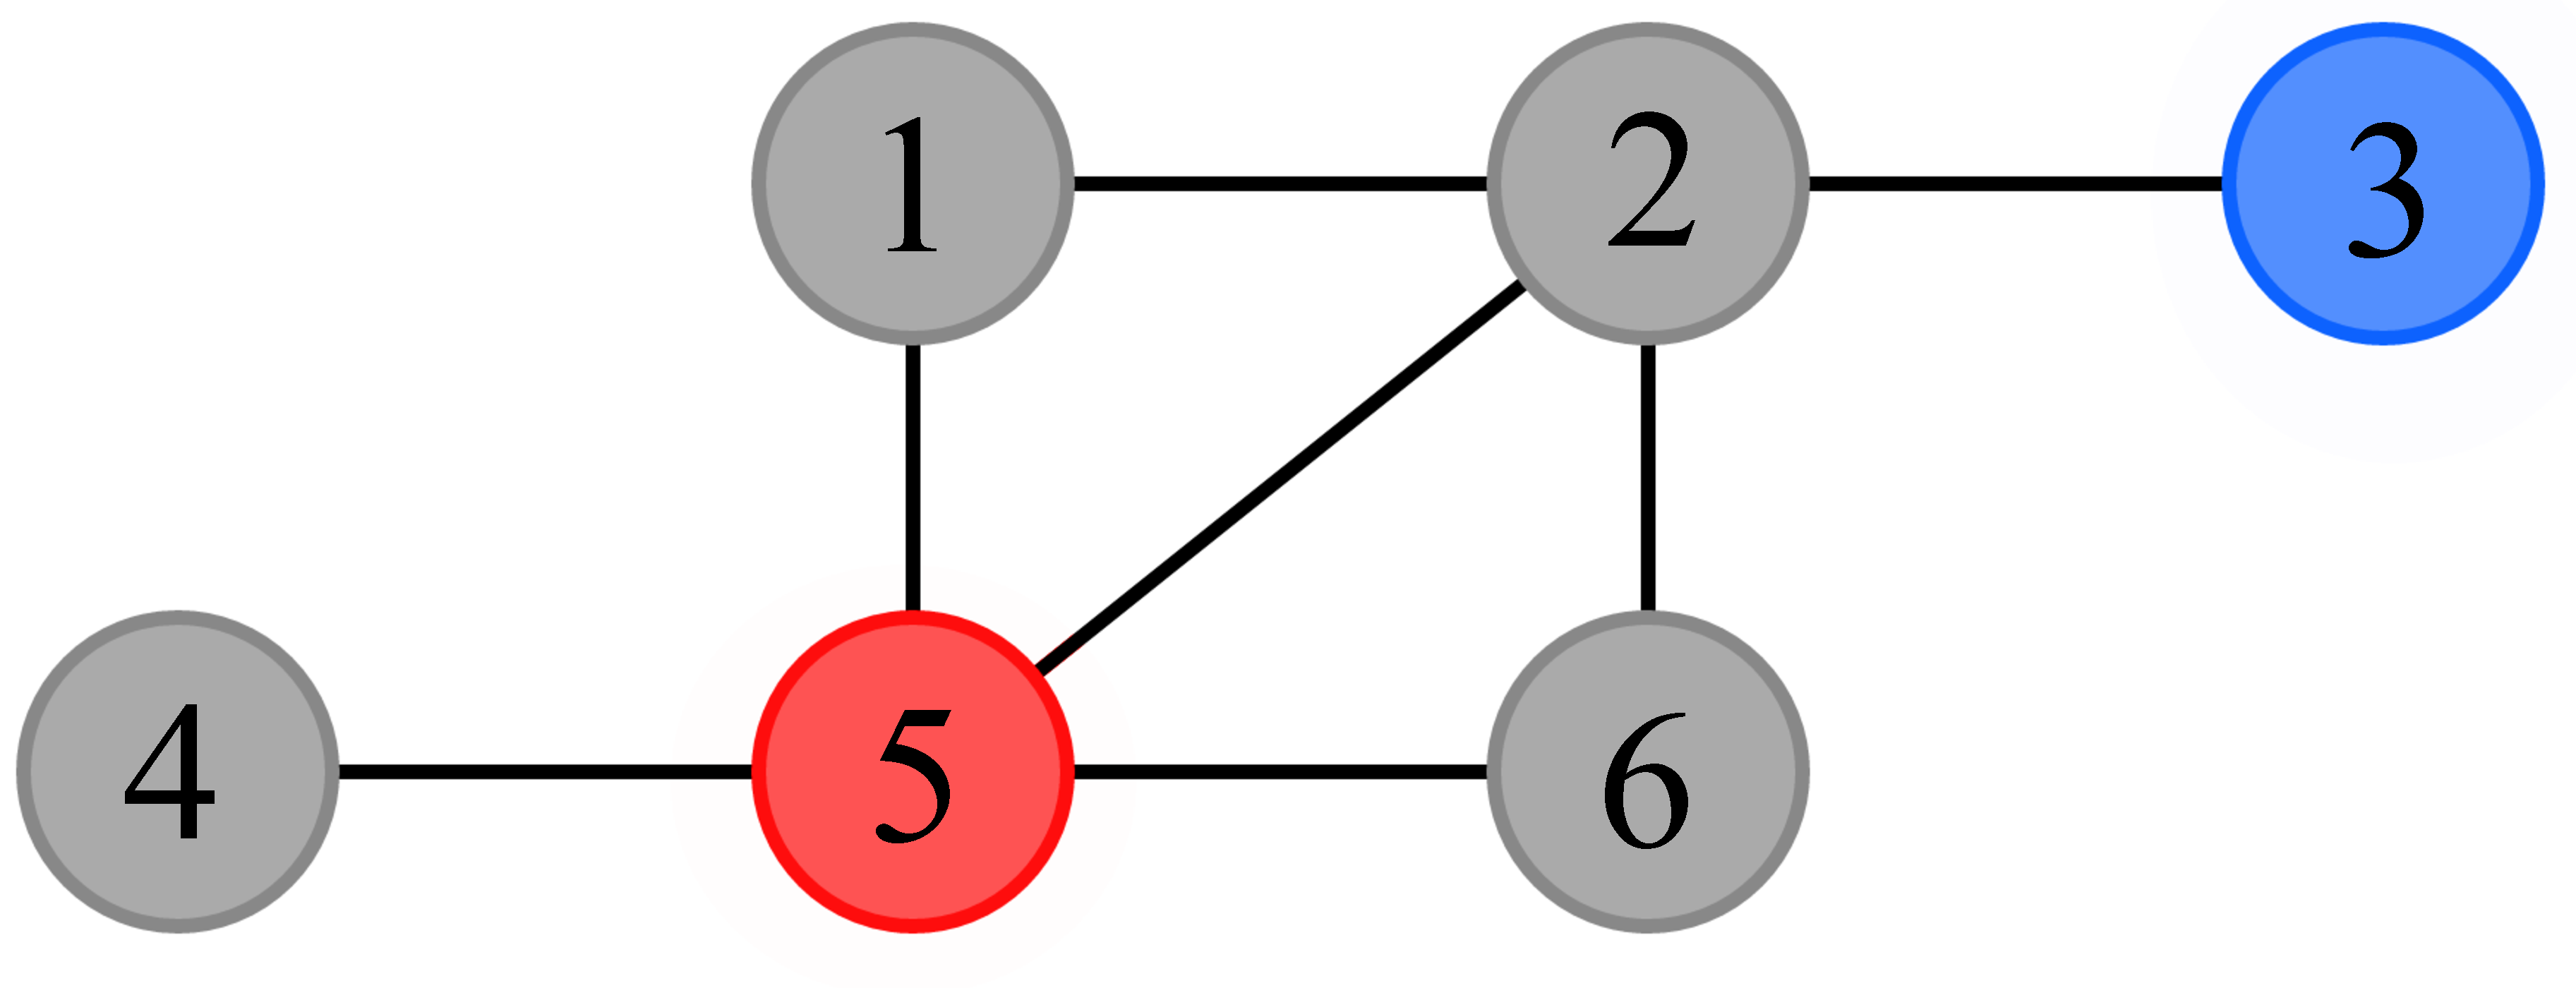
\includegraphics[width=8cm]{../figures/example-cfcp.pdf}
    \end{textblock*}

    \vspace{4cm}
    \vfill

    \begin{itemize}
      \item<1-2> A \textbf{conflict-free coloring} of a graph $G$ assigns colors to \emph{some} vertices such that there is a uniquely colored vertex within the neighborhood of every vertex.
      \item<2> Every proper vertex coloring of $G$ is also a conflict-free coloring of $G$ as every vertex $v$ would be a unique color itself in its neighborhood.
    \end{itemize}
  \end{frame}

  \begin{frame}
    \frametitle{Conflict-Free Coloring}

    \begin{textblock*}{\examplewidth/2}(0cm,\exampleheight) % {block width} (coords)
      \centering
      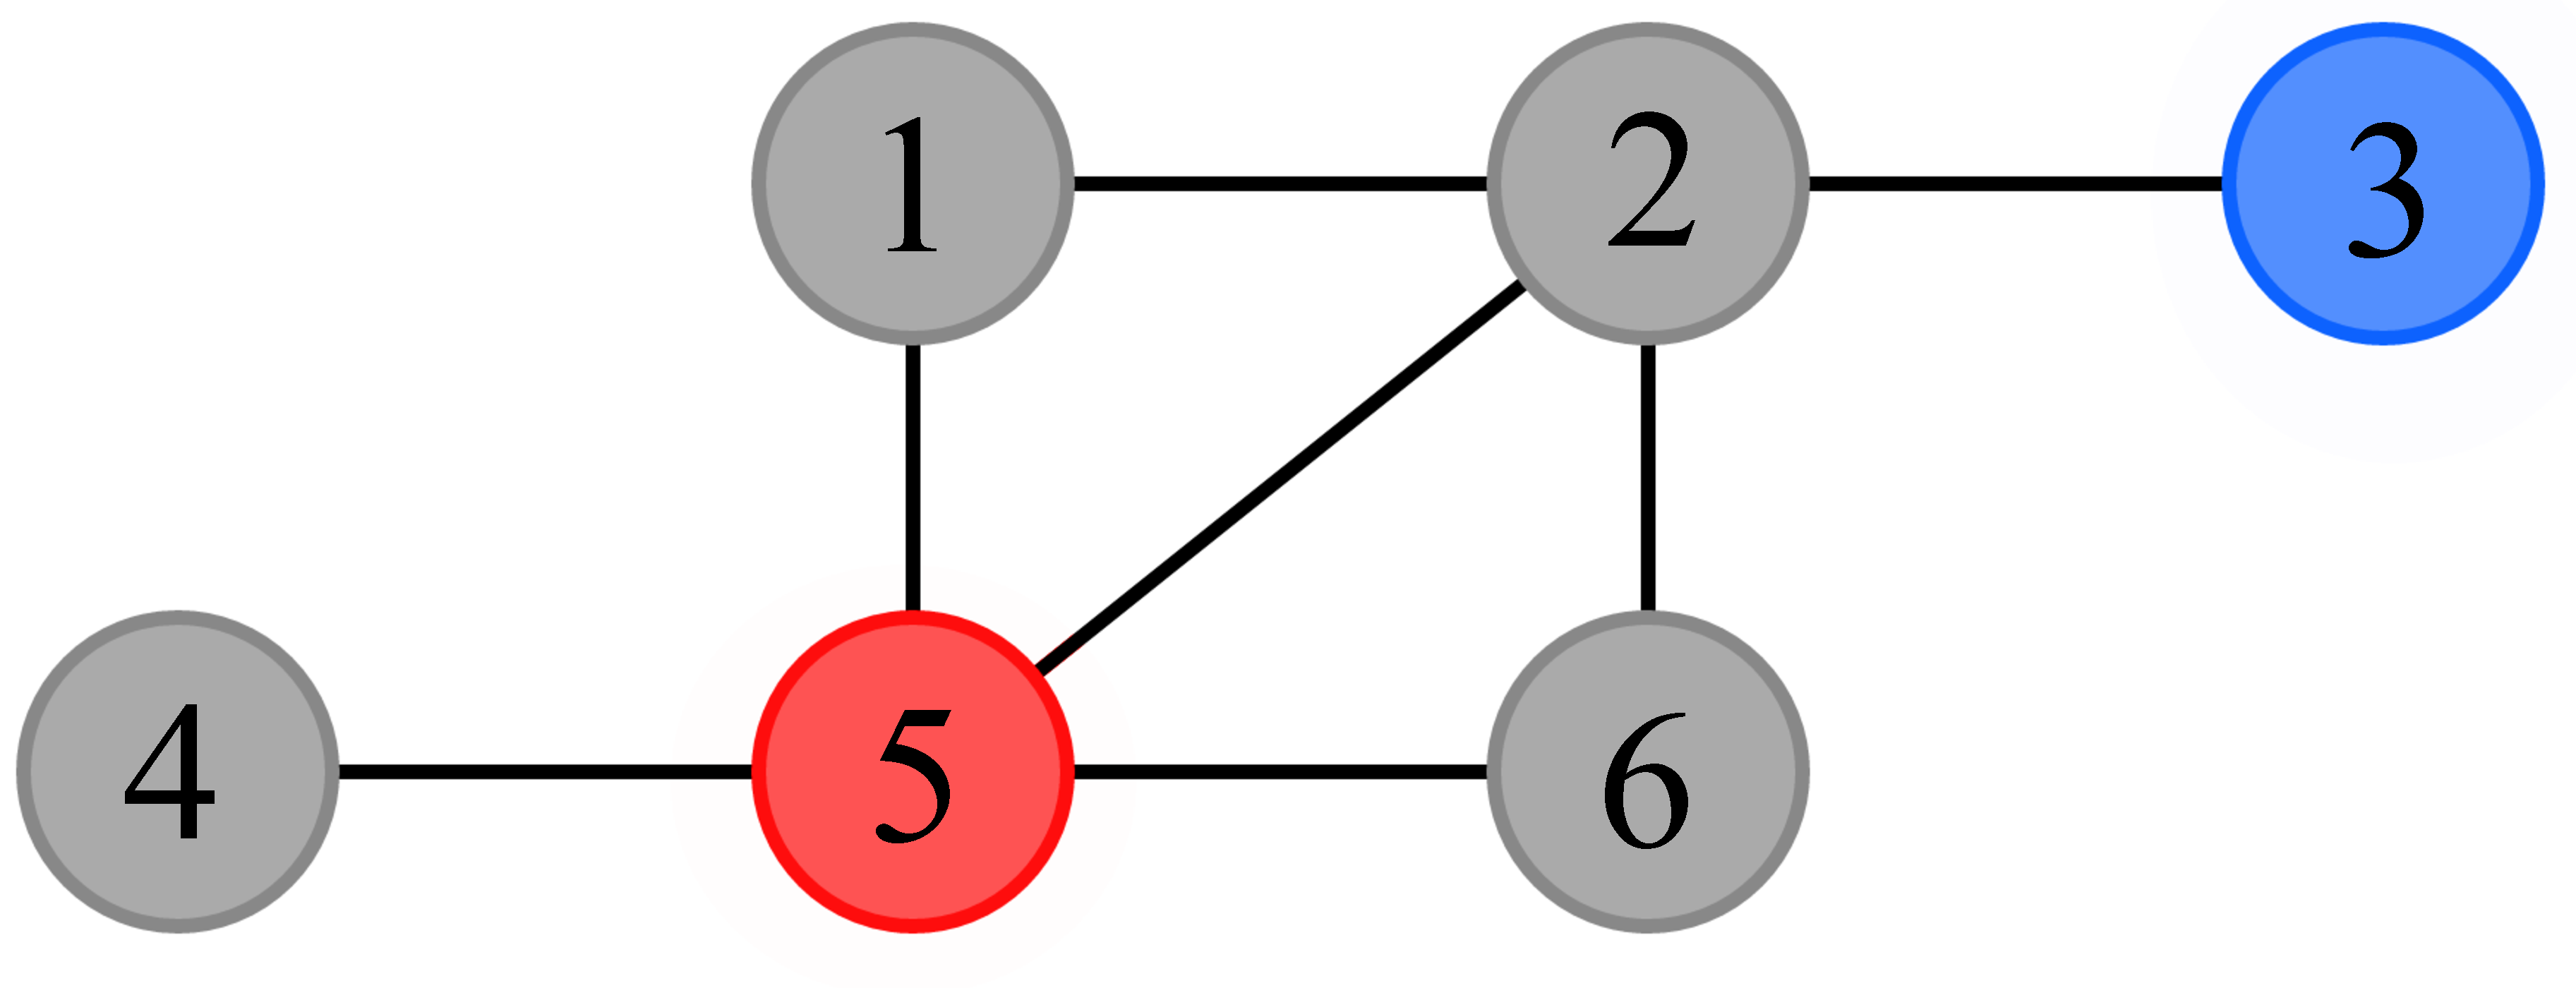
\includegraphics[width=6.5cm]{../figures/example-cfcp.pdf}
    \end{textblock*}

    \begin{textblock*}{\examplewidth/2}(8cm,\exampleheight) % {block width} (coords)
      \centering
      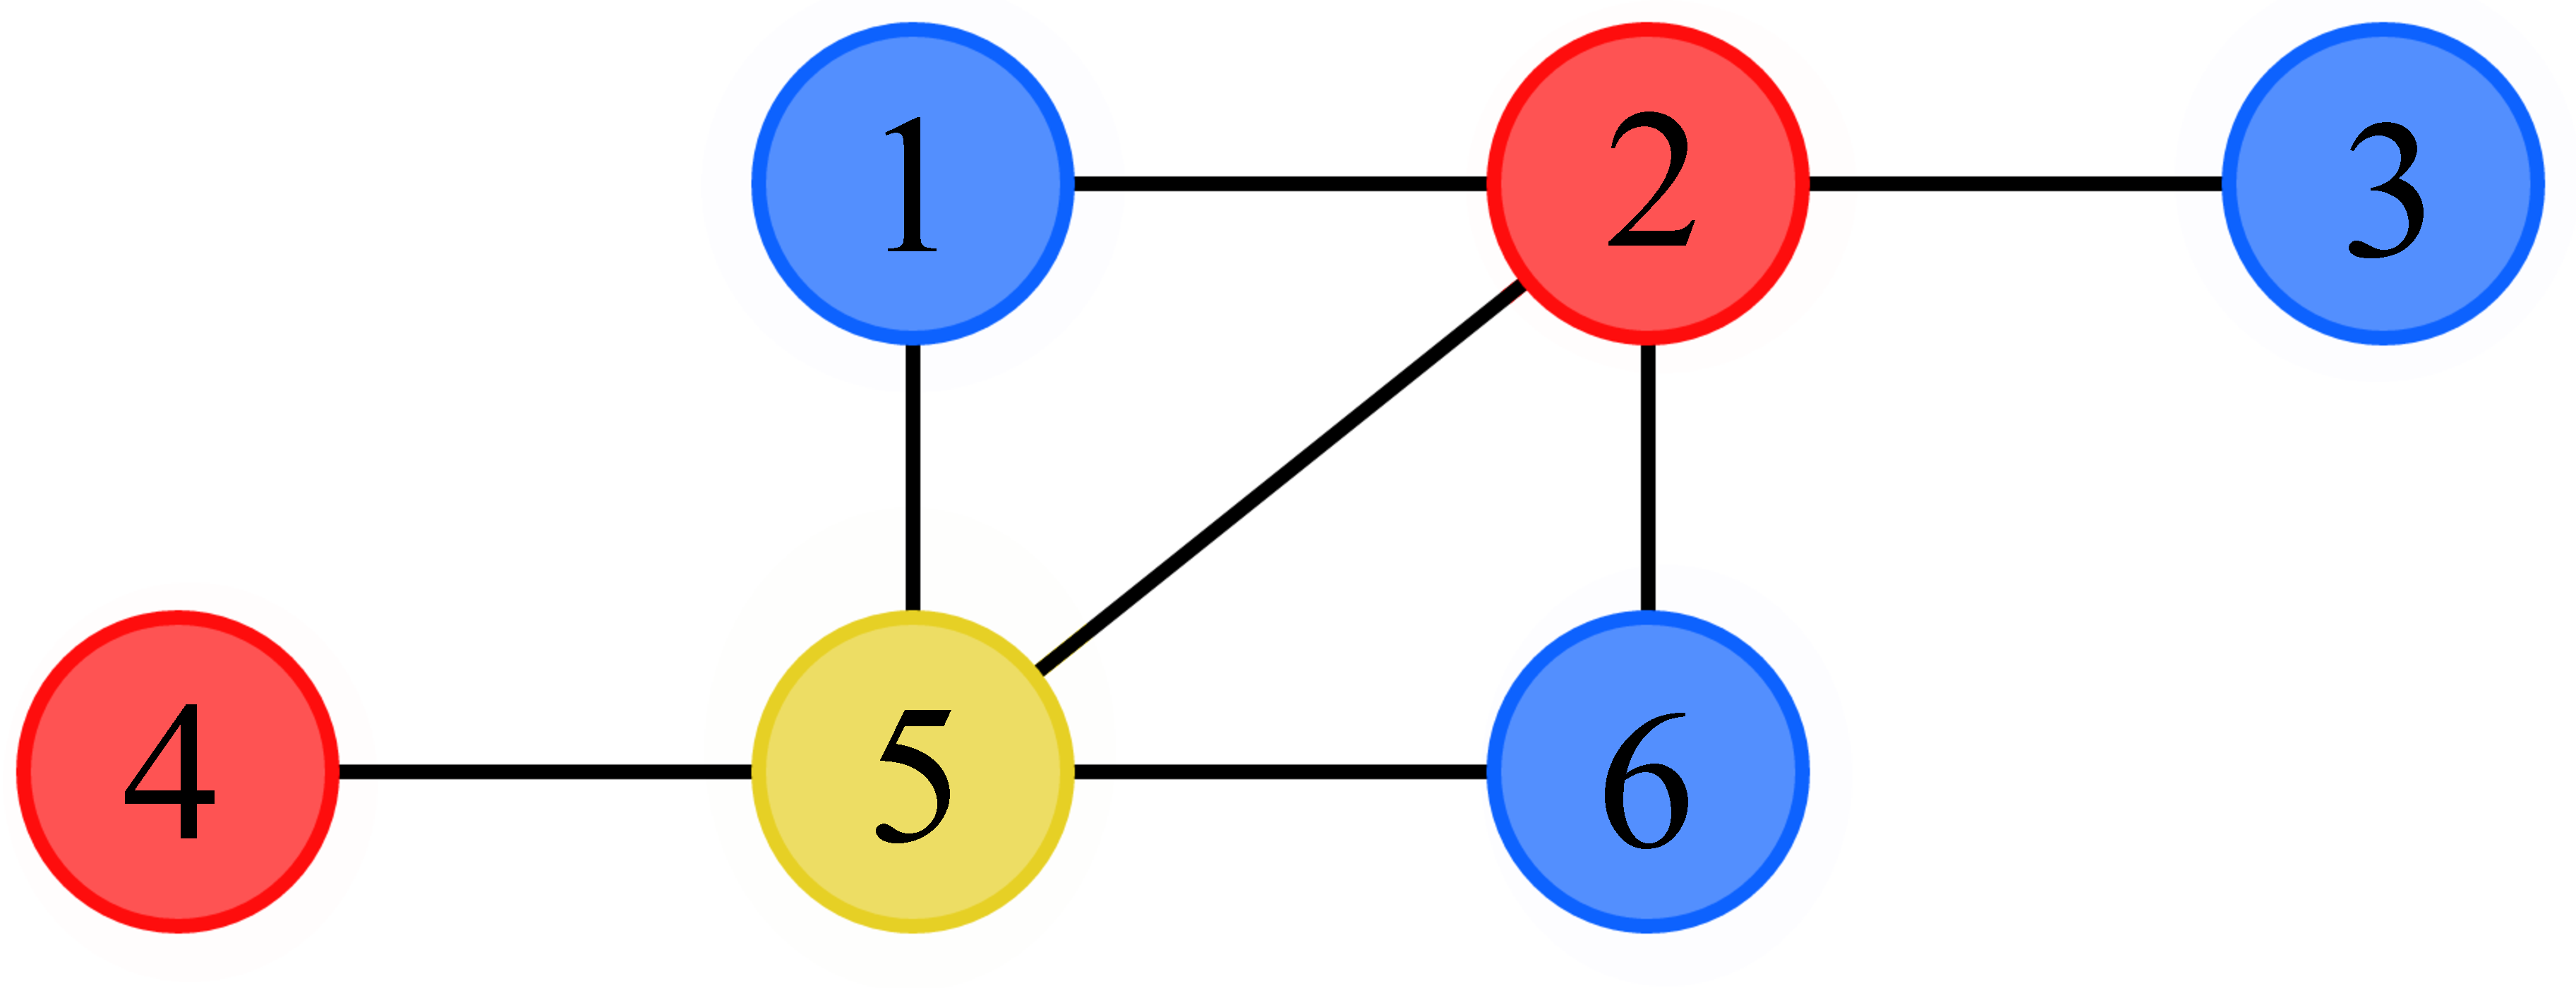
\includegraphics[width=6.5cm]{../figures/example-vcp.pdf}
    \end{textblock*}

    \vspace{3cm}

    \begin{center}
      Every vertex $v$ has at least one unique color within its neighborhood.
    \end{center}

    \pause

    \begin{columns}
      \begin{column}{0.5\textwidth}
        \begin{itemize}[leftmargin=1.4cm]
          \item[$v$ = 1:] $\{1: none,\ 2: none,\ 5: \textbf{red}\}$
          \item[$v$ = 2:] $\{1: none,\ 2: none,\ 3: \textbf{blue},$ \newline $\quad 5: red,\ 6: none\}$
          \item[$v$ = 3:] $\{2: none,\ 3: \textbf{blue}\}$
        \end{itemize}
      \end{column}

      \pause

      \begin{column}{0.5\textwidth}
        \begin{itemize}[leftmargin=1.4cm]
          \item[$v$ = 1:] $\{1: \textbf{blue},\ 2: red,\ 5: yellow\}$
          \item[$v$ = 2:] $\{1: blue,\ 2: \textbf{red},\ 3: blue,$ \newline $\quad 5: yellow,\ 6: blue\}$
          \item[$v$ = 3:] $\{2: red,\ 3: \textbf{blue}\}$
        \end{itemize}
      \end{column}
    \end{columns}

  \end{frame}

  \begin{frame}
    \frametitle{Conflict-Free Coloring Examples}

    \begin{textblock*}{\examplewidth}(1cm,\exampleheight) % {block width} (coords)
      Incorrect conflict-free colorings and their fixes:
    \end{textblock*}

    \vspace{0.5cm}

    \pause

    \begin{columns}
      \begin{column}{0.33333\textwidth}
        \only<2>{
          \begin{figure}[h]
            \centering
            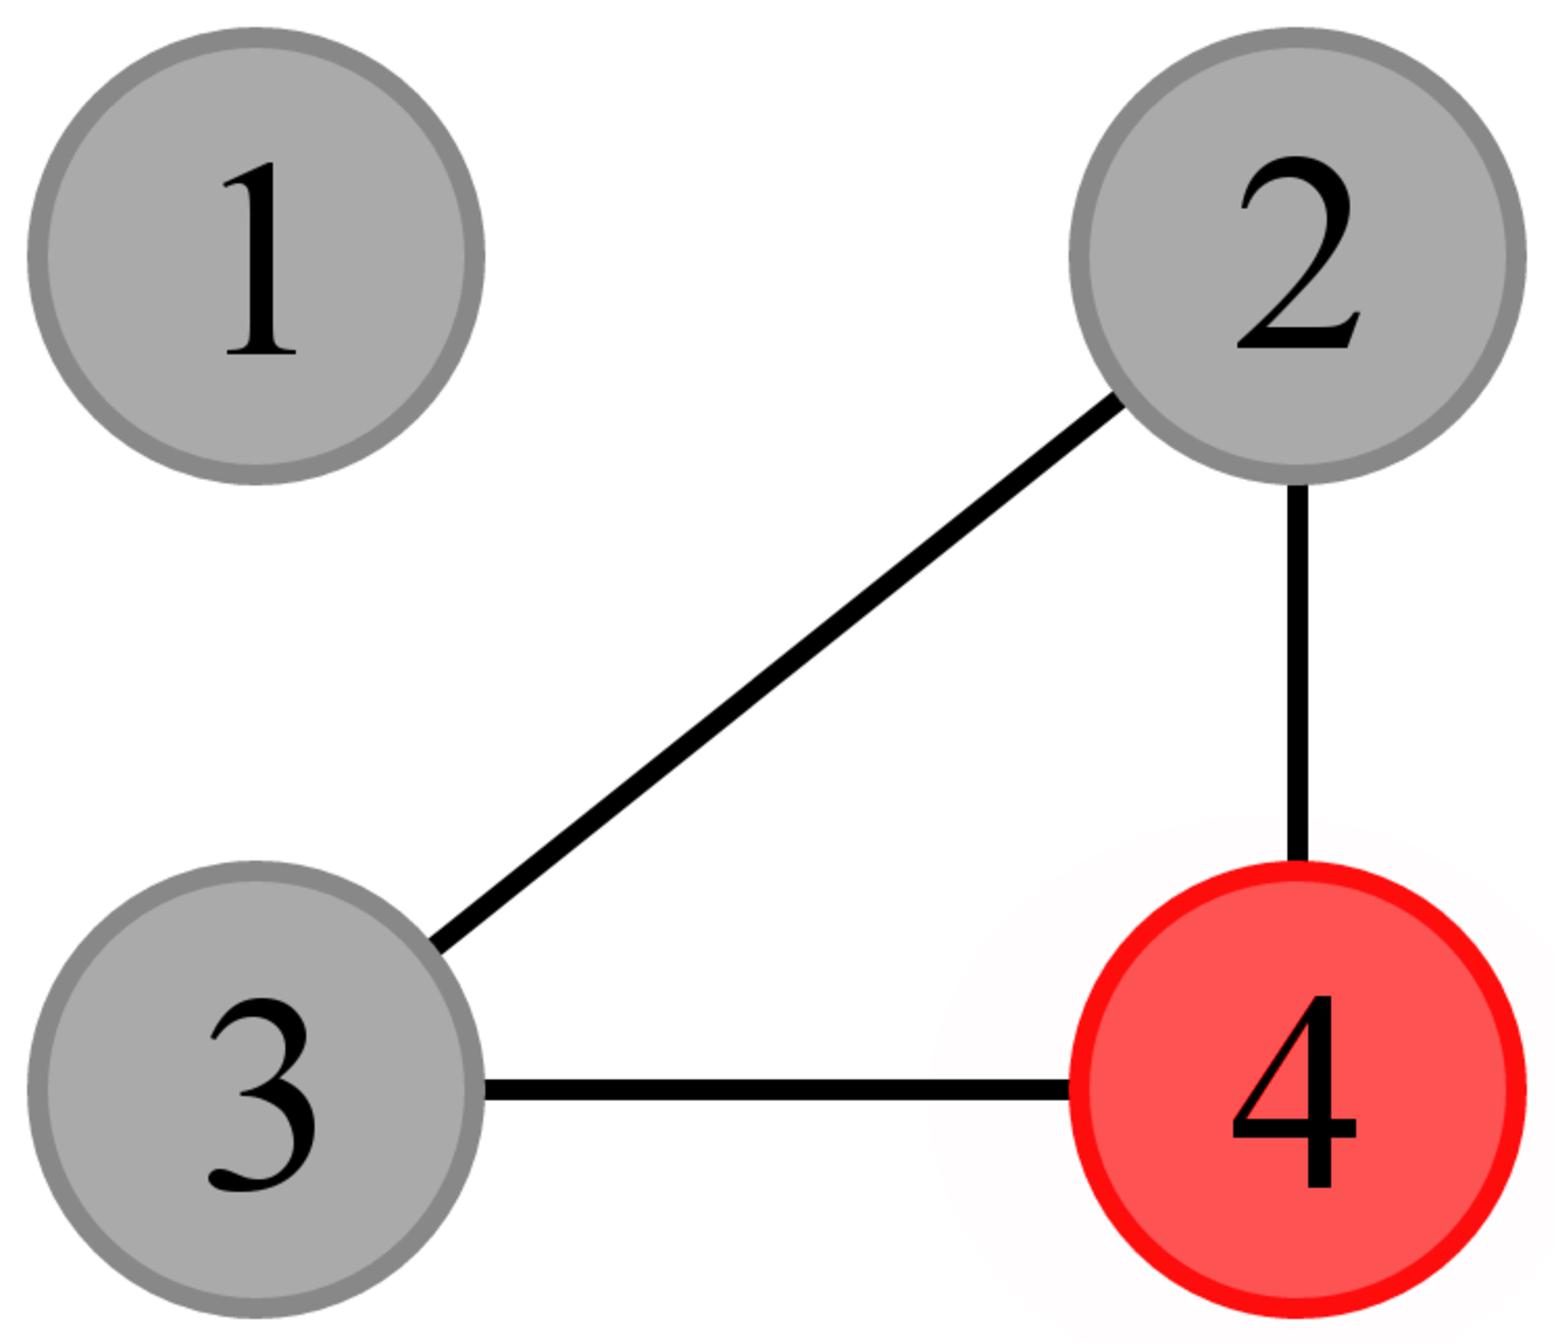
\includegraphics[width=3cm]{../figures/examples-1-incorrect-1.pdf}
          \end{figure}
        }

        \only<3-7>{
          \begin{figure}[h]
            \centering
            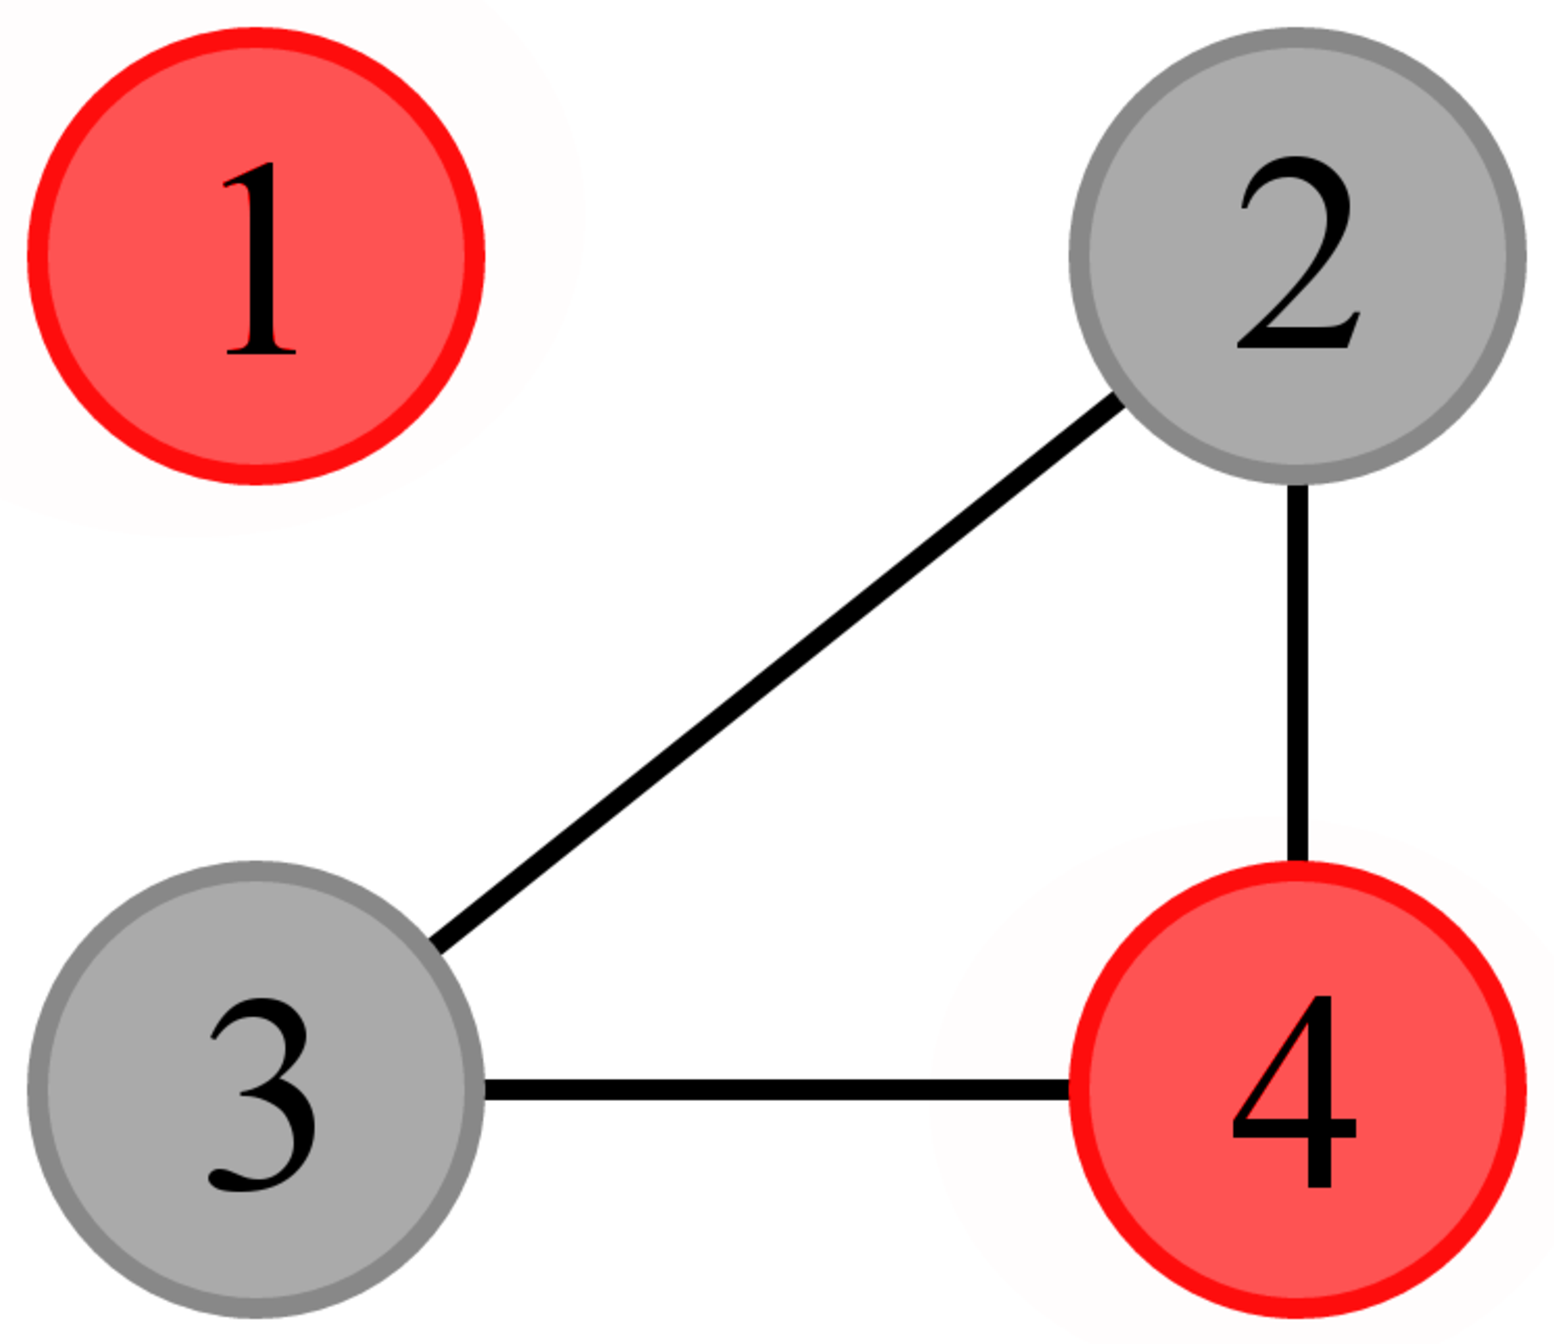
\includegraphics[width=3cm]{../figures/examples-1-incorrect-1-corrected.pdf}
          \end{figure}
        }

        \centering
        Vertex 1 does not have a unique color in its neighborhood.
      \end{column}

      \pause
      \pause

      \begin{column}{0.33333\textwidth}

        \only<4>{
        \begin{figure}[h]
          \centering
          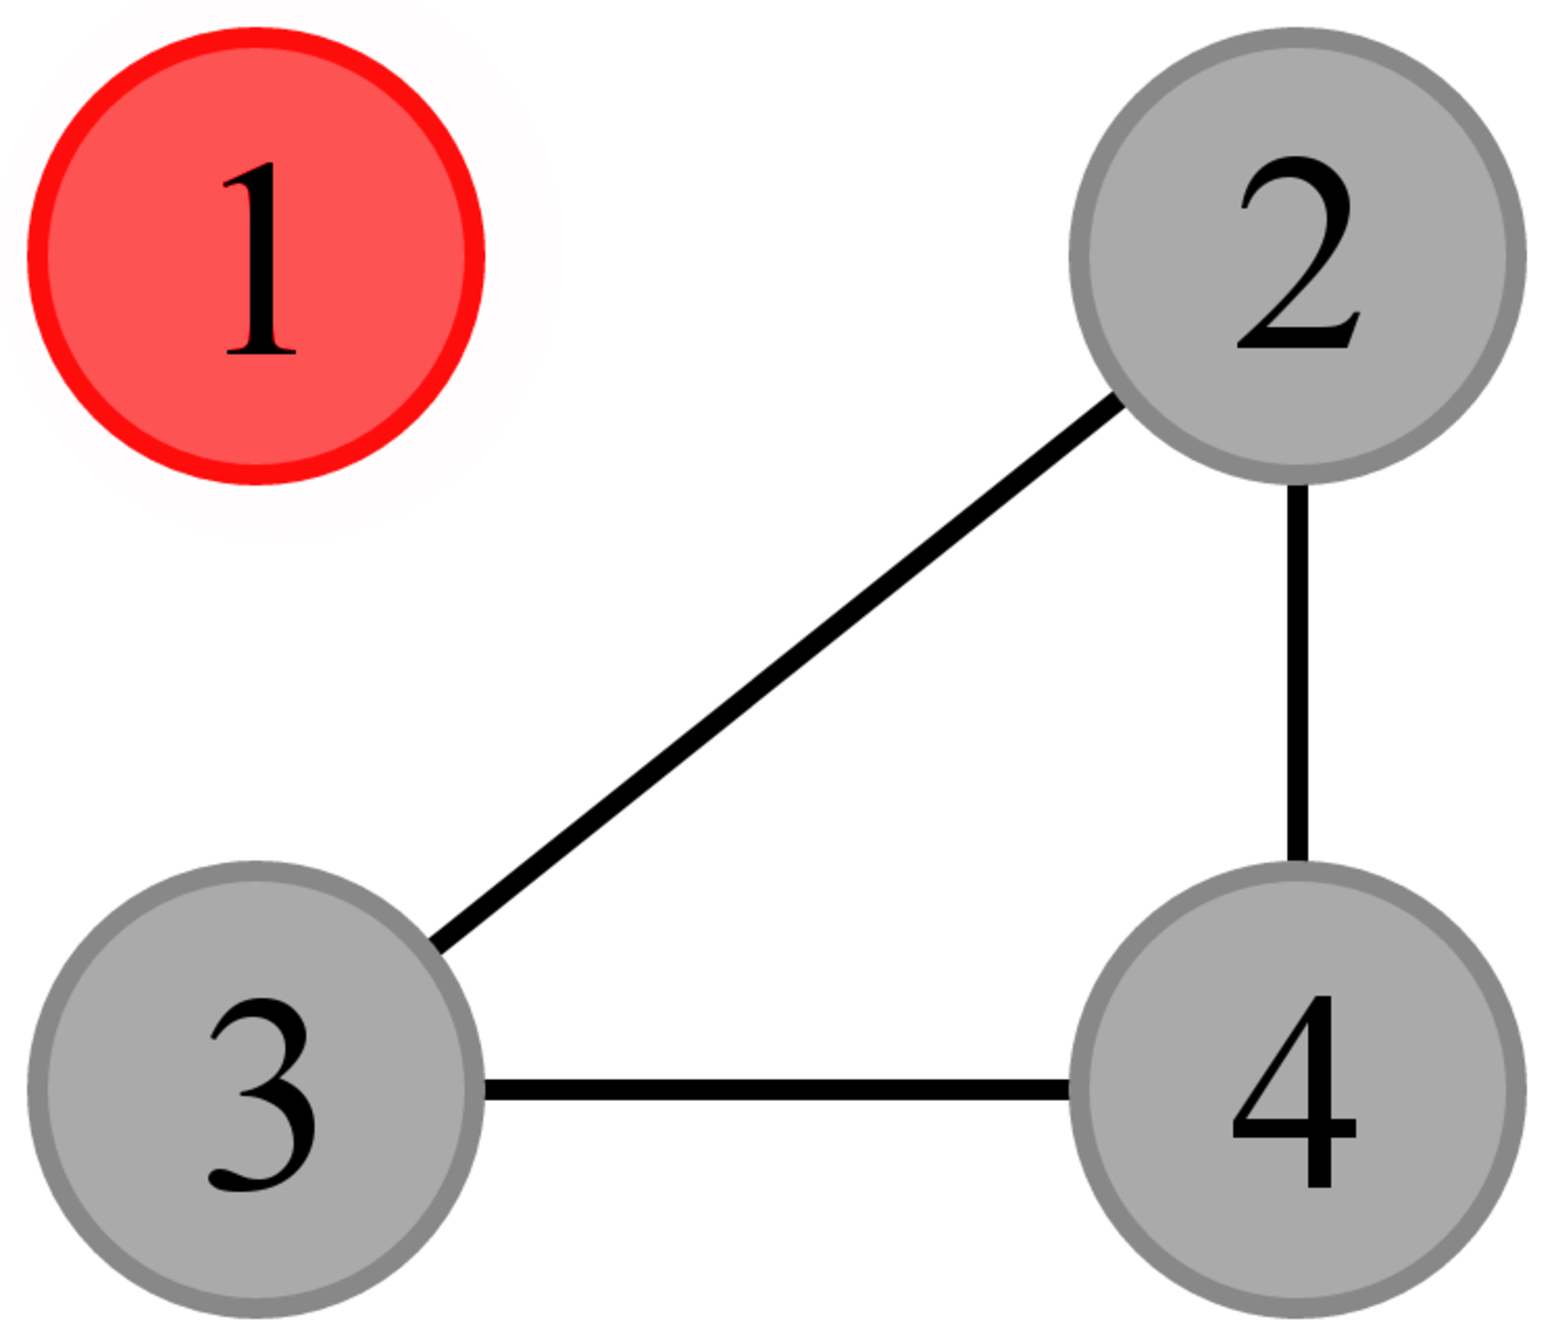
\includegraphics[width=3cm]{../figures/examples-1-incorrect-2.pdf}
        \end{figure}
        }

        \only<5-7>{
        \begin{figure}[h]
          \centering
          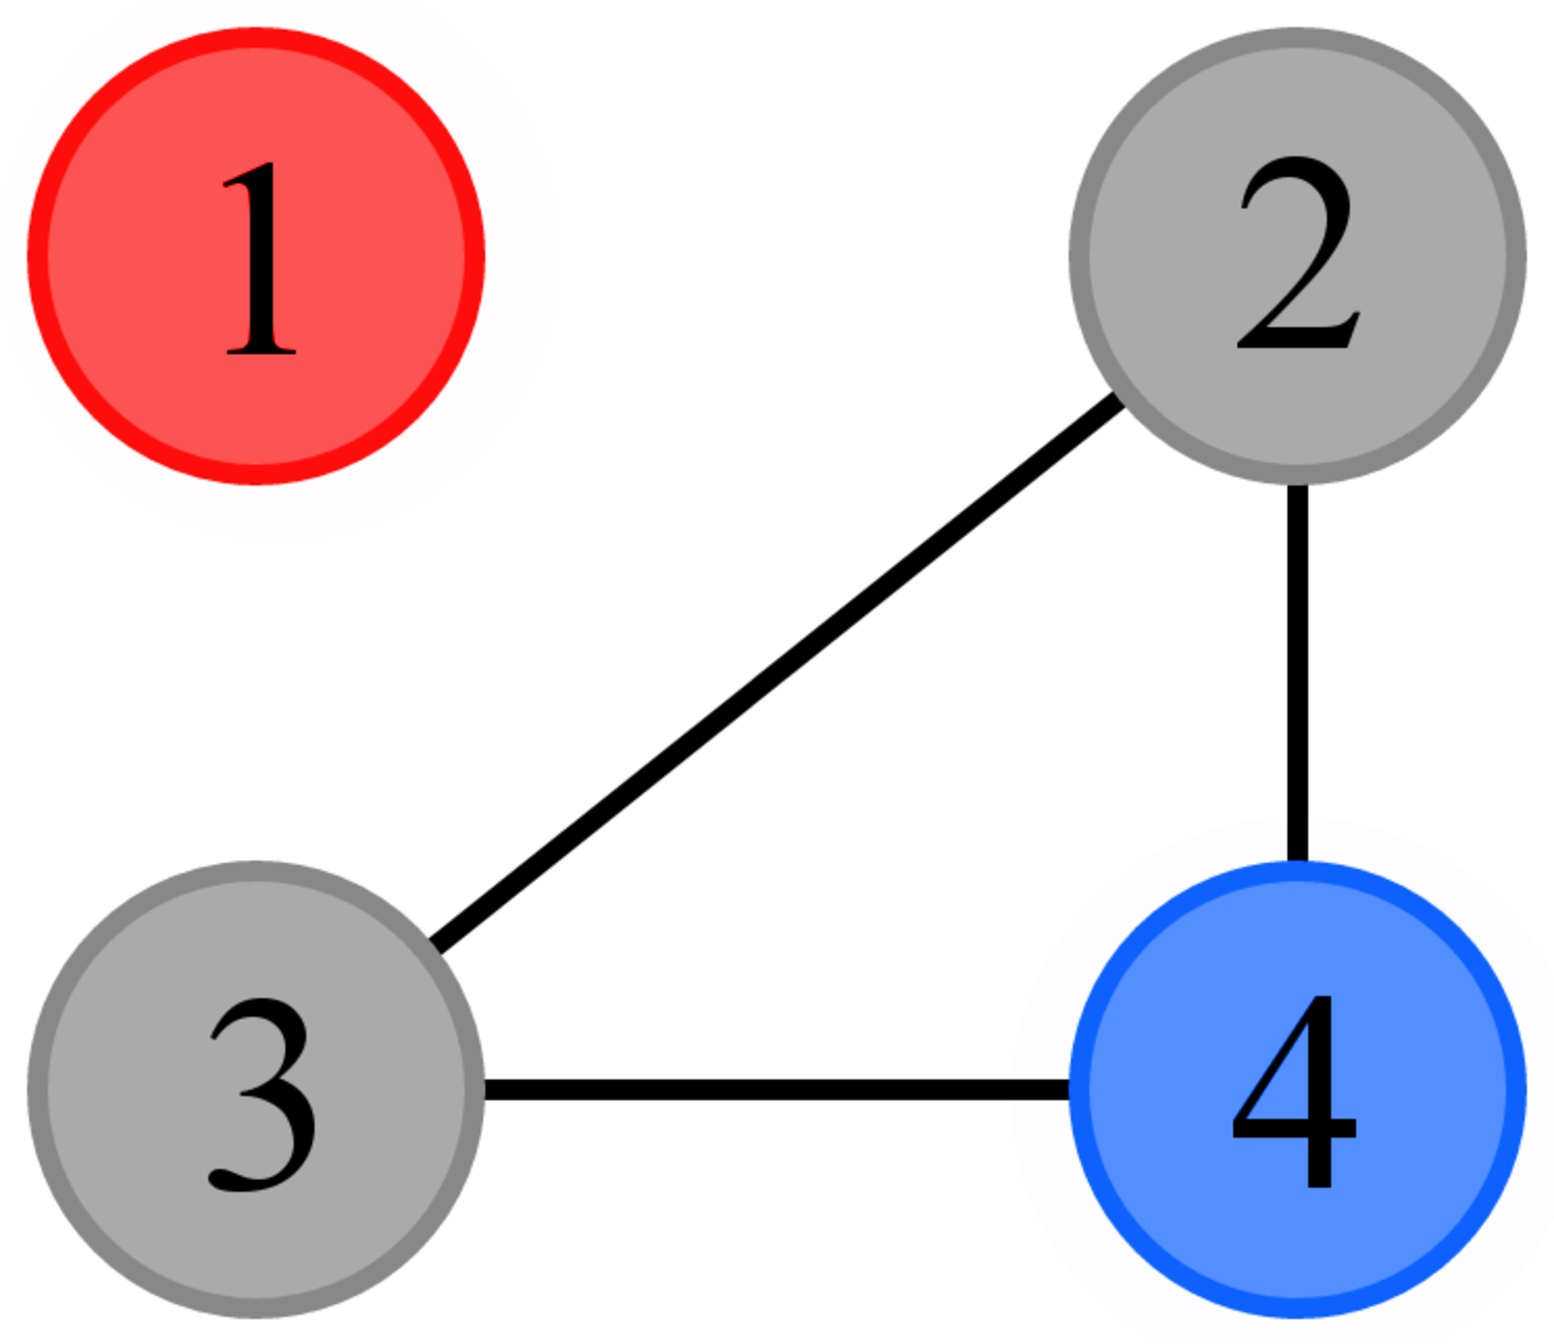
\includegraphics[width=3cm]{../figures/examples-1-incorrect-2-corrected.pdf}
        \end{figure}
        }

        \centering
        Vertices $\{2, 3, 4\}$ do not have a unique color in their neighborhoods.
      \end{column}

      \pause
      \pause

      \begin{column}{0.33333\textwidth}

        \only<6>{
        \begin{figure}[h]
          \centering
          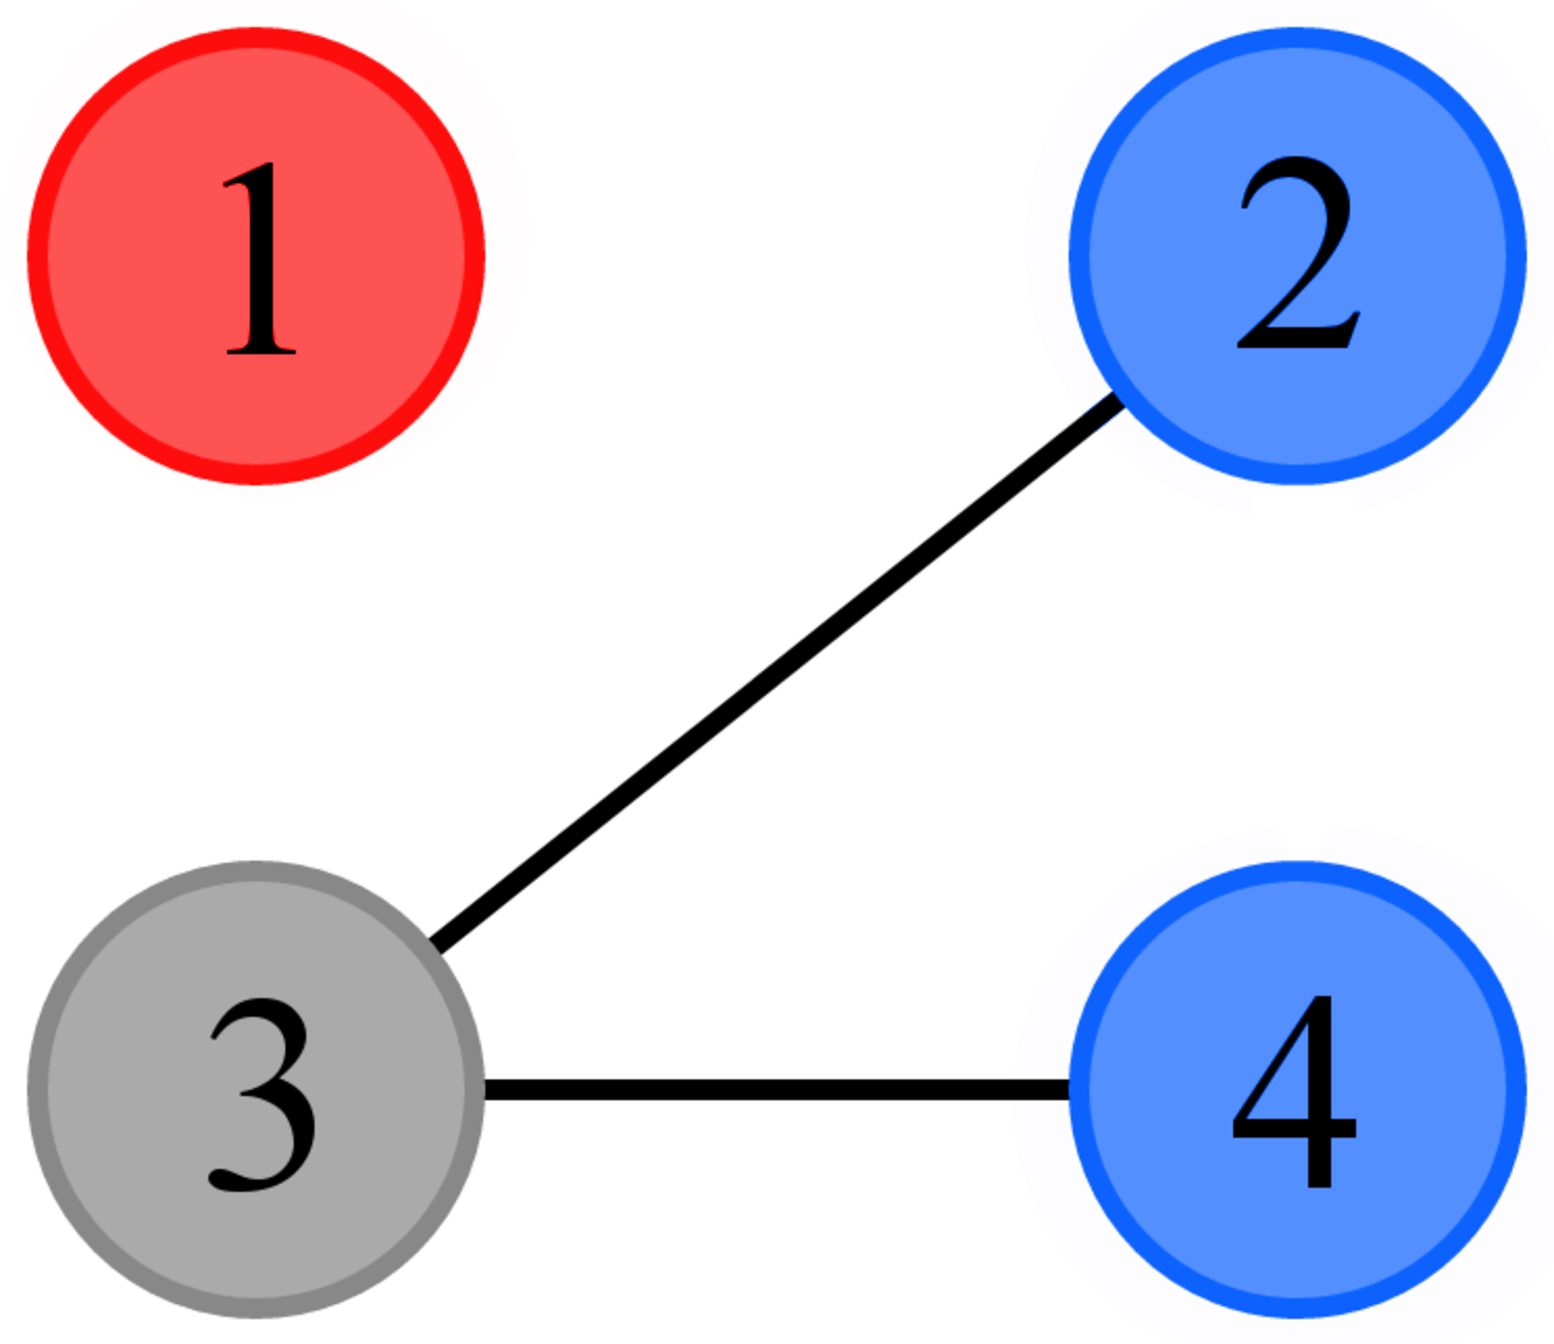
\includegraphics[width=3cm]{../figures/examples-1-incorrect-3.pdf}
        \end{figure}
        }

        \only<7>{
        \begin{figure}[h]
          \centering
          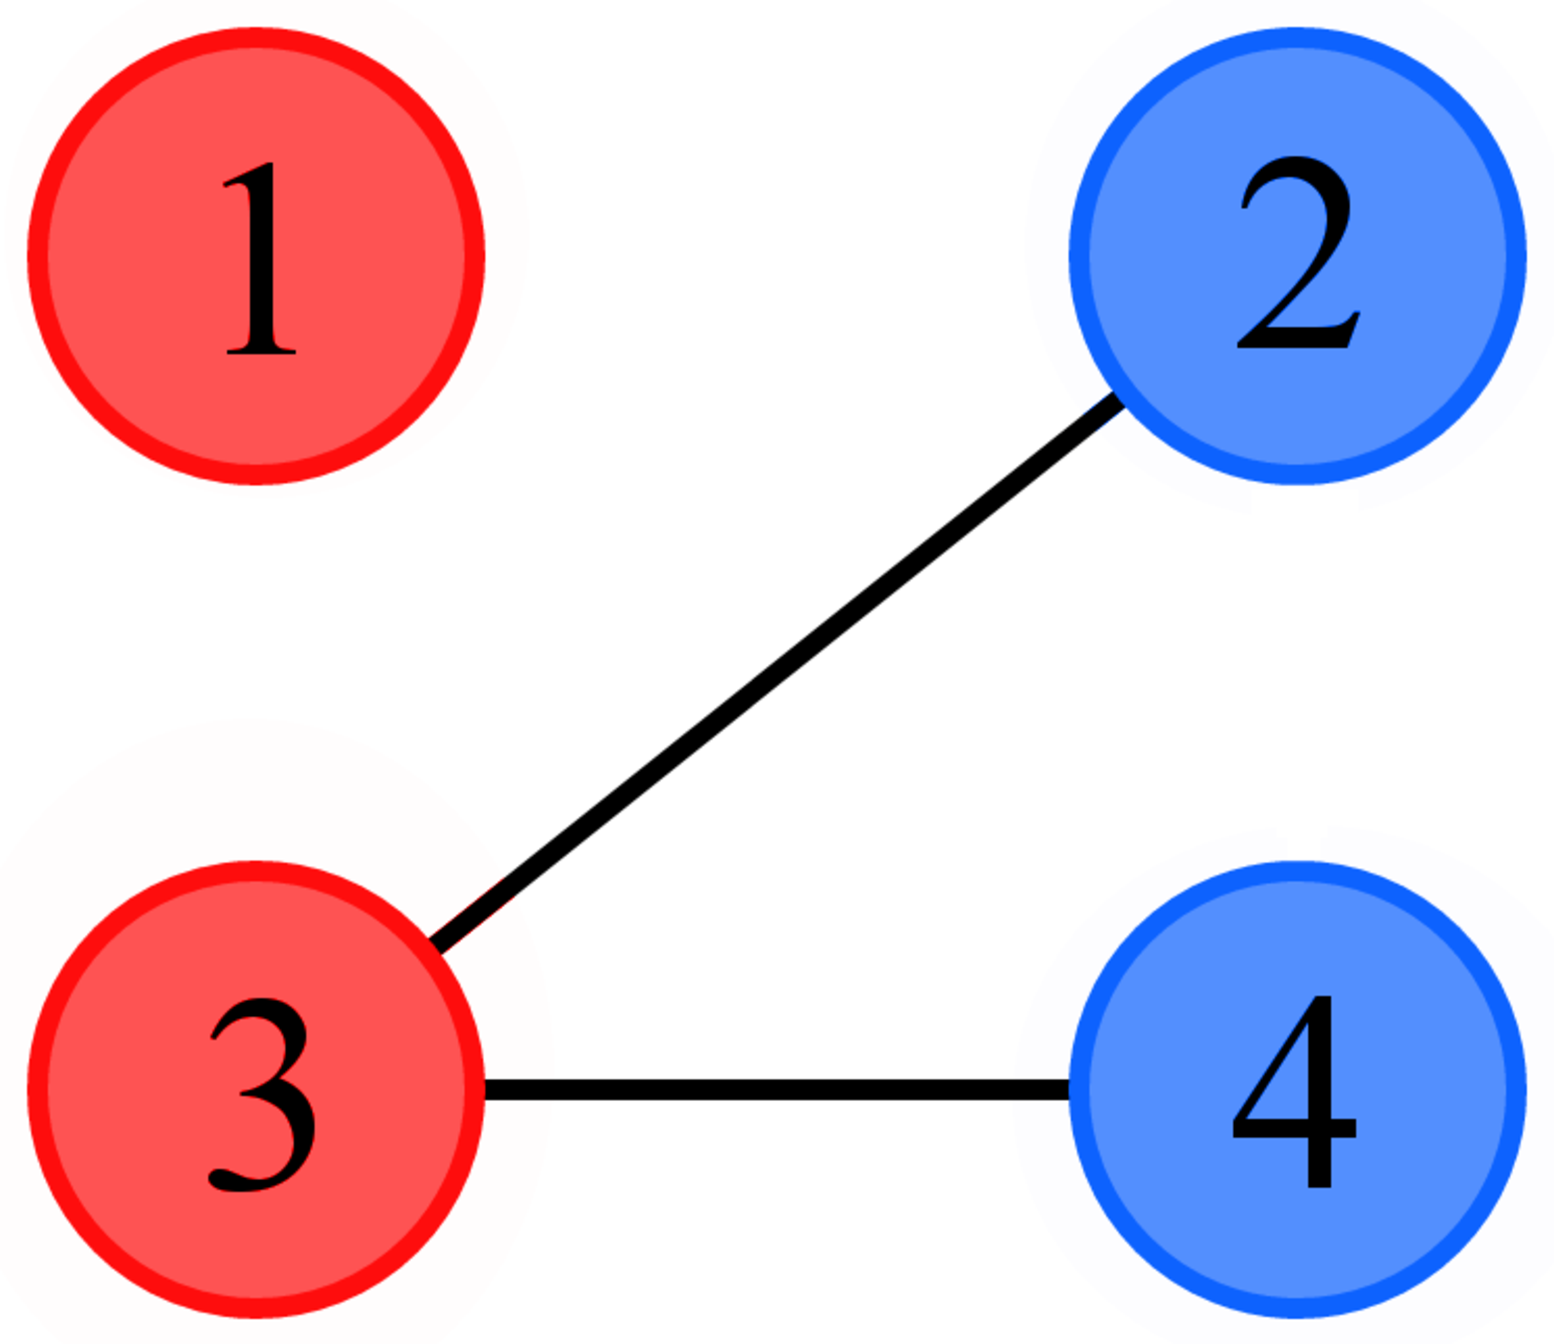
\includegraphics[width=3cm]{../figures/examples-1-incorrect-3-corrected.pdf}
        \end{figure}
        }

        \centering
        Vertex 3 does not have a unique color in its neighborhood.
      \end{column}
    \end{columns}

  \end{frame}

  \addtocontents{toc}{\protect\vspace{14pt}}

  \section{Applications}

  \subsection{Wireless Networks}

  \begin{frame}
    \frametitle{Wireless Networks}

    \begin{itemize}
      \item \textbf{Wireless networks} such as cellular networks, television broadcasts, and satellite communication systems can all benefit from conflict-free coloring.

      \begin{figure}[h]
        \centering
        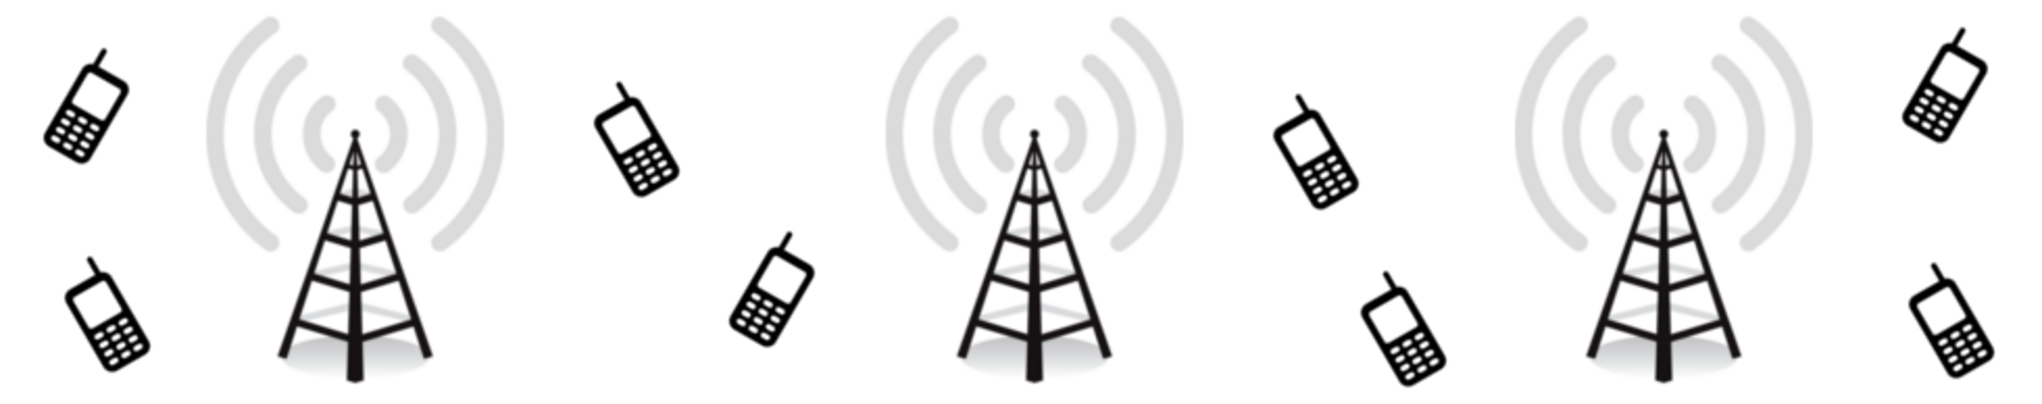
\includegraphics[width=12cm]{../figures/towers-slides.pdf}
      \end{figure}

      \pause

      \item A \textbf{cellular network} is a heterogeneous network with two types of nodes.

      \pause

      \begin{itemize}
        \item Base-stations act as servers and are interconnected by an external backbone network.
        \pause
        \item Clients connect to base-stations via radio links. They constantly search for base-stations with strong reception.
      \end{itemize}
    \end{itemize}

  \end{frame}

  \begin{frame}
    \frametitle{Cellular Networks}

    \begin{itemize}
      \item The problem when designing cellular networks: \textbf{frequency assignment}.
      \begin{itemize}
        \item Imagine two nearby base-stations having the same frequency.
        \item A client in range of both base-stations would receive mutual interference.
      \end{itemize}
    \end{itemize}

    \pause
    \vspace{-0.2cm}

    \begin{itemize}
      \item This leads us to our goal: Assign frequencies such that:
      \pause
      \begin{itemize}
        \item[(1)] Every client is served by a base-station with a unique frequency
        \pause
        \item[(2)] Minimize the number of frequencies used
      \end{itemize}
    \end{itemize}

    \pause
    \vfill

    \begin{figure}[h]
      \centering
      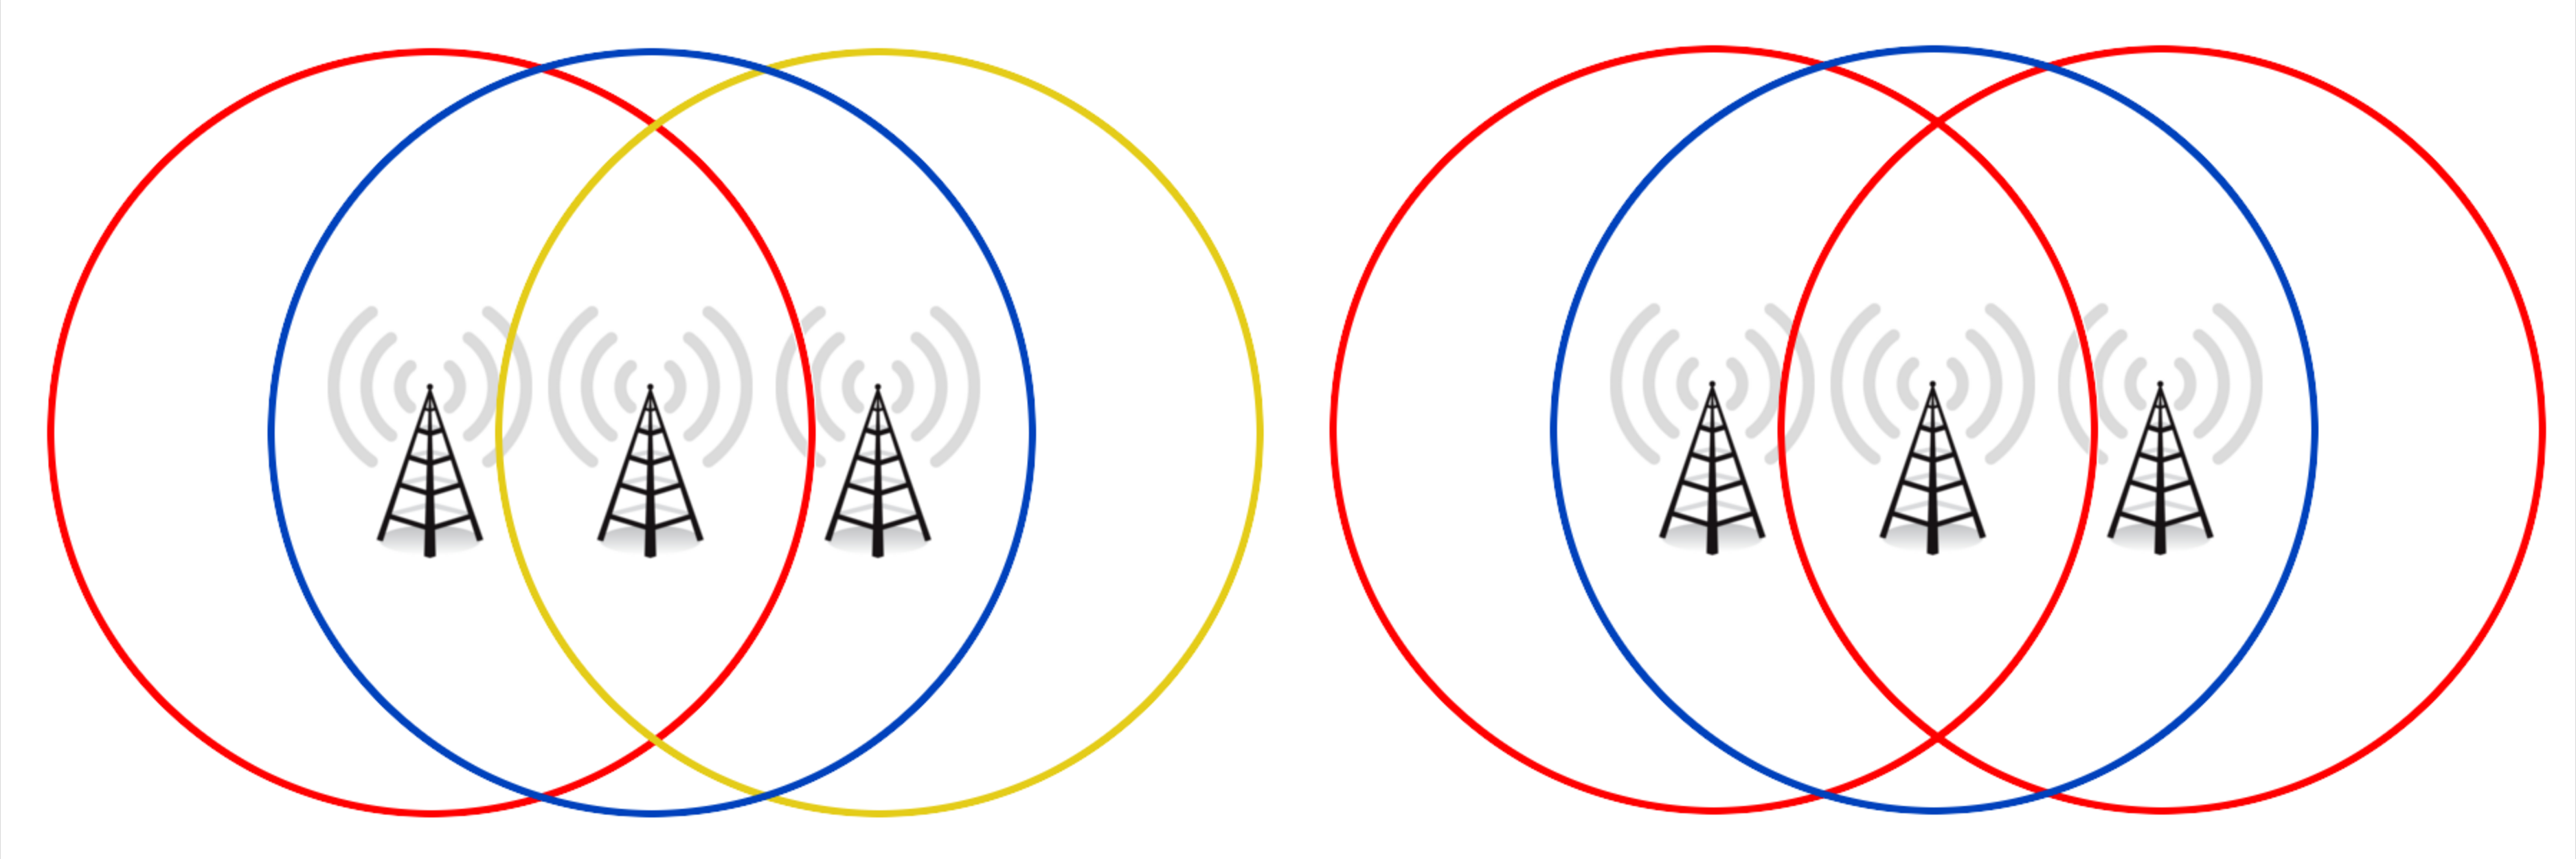
\includegraphics[width=8cm,trim=4 4 4 4,clip]{../figures/towers.pdf}
      \caption{Vertex coloring and conflict-free coloring of cellular towers, respectively}
    \end{figure}

  \end{frame}

  \subsection{RFID Networks}

  \begin{frame}
    \frametitle{RFID Networks}
  \end{frame}

  \addtocontents{toc}{\newpage}

  \section{CF Coloring for General Graphs}
  \subsection{Guaranteeing CF k-Colorability}
  \begin{frame}
    \frametitle{Guaranteeing Conflict-Free k-Colorability}

    It is wasteful to spend time coloring a graph that cannot be conflict-free colored within a certain amount of colors ($k$). Thus researchers came up with a criterion to guarantee a graph can be colored with $k$ colors.

    \pause
    \vfill

    A \textbf{complete graph} is a graph where every pair of distinct vertices is connected by an edge.

    \pause

    \begin{itemize}
      \item $K_n$: A complete graph of $n$ vertices.
      \pause
      \item $K_n^{-3}$: A complete graph of $n$ vertices with any three edges forming a triangle removed.
    \end{itemize}

    \pause
    \vfill

    \begin{theorem}
    Let $G$ be a graph and $k \geq 1$. If $G$ has neither $K_{k+2}$ nor $K_{k+3}^{-3}$ as a minor, $G$ has a conflict-free coloring that can be found in polynomial time.
    \end{theorem}

  \end{frame}

  \begin{frame}
    \frametitle{Guaranteeing Conflict-Free k-Colorability}

    % \begin{textblock*}{\examplewidth}(1cm,1.4cm) % {block width} (coords)
    % \end{textblock*}




    \begin{textblock*}{14cm}(1cm, 1.6cm) % {block width} (coords)
      Let's demonstrate meeting this criterion on a graph for the simplest case, $k=1$:
    \end{textblock*}


    \begin{textblock*}{15cm}(0.5cm, 2.1cm) % {block width} (coords)
      \only<1>{
        \begin{figure}
         \centering
         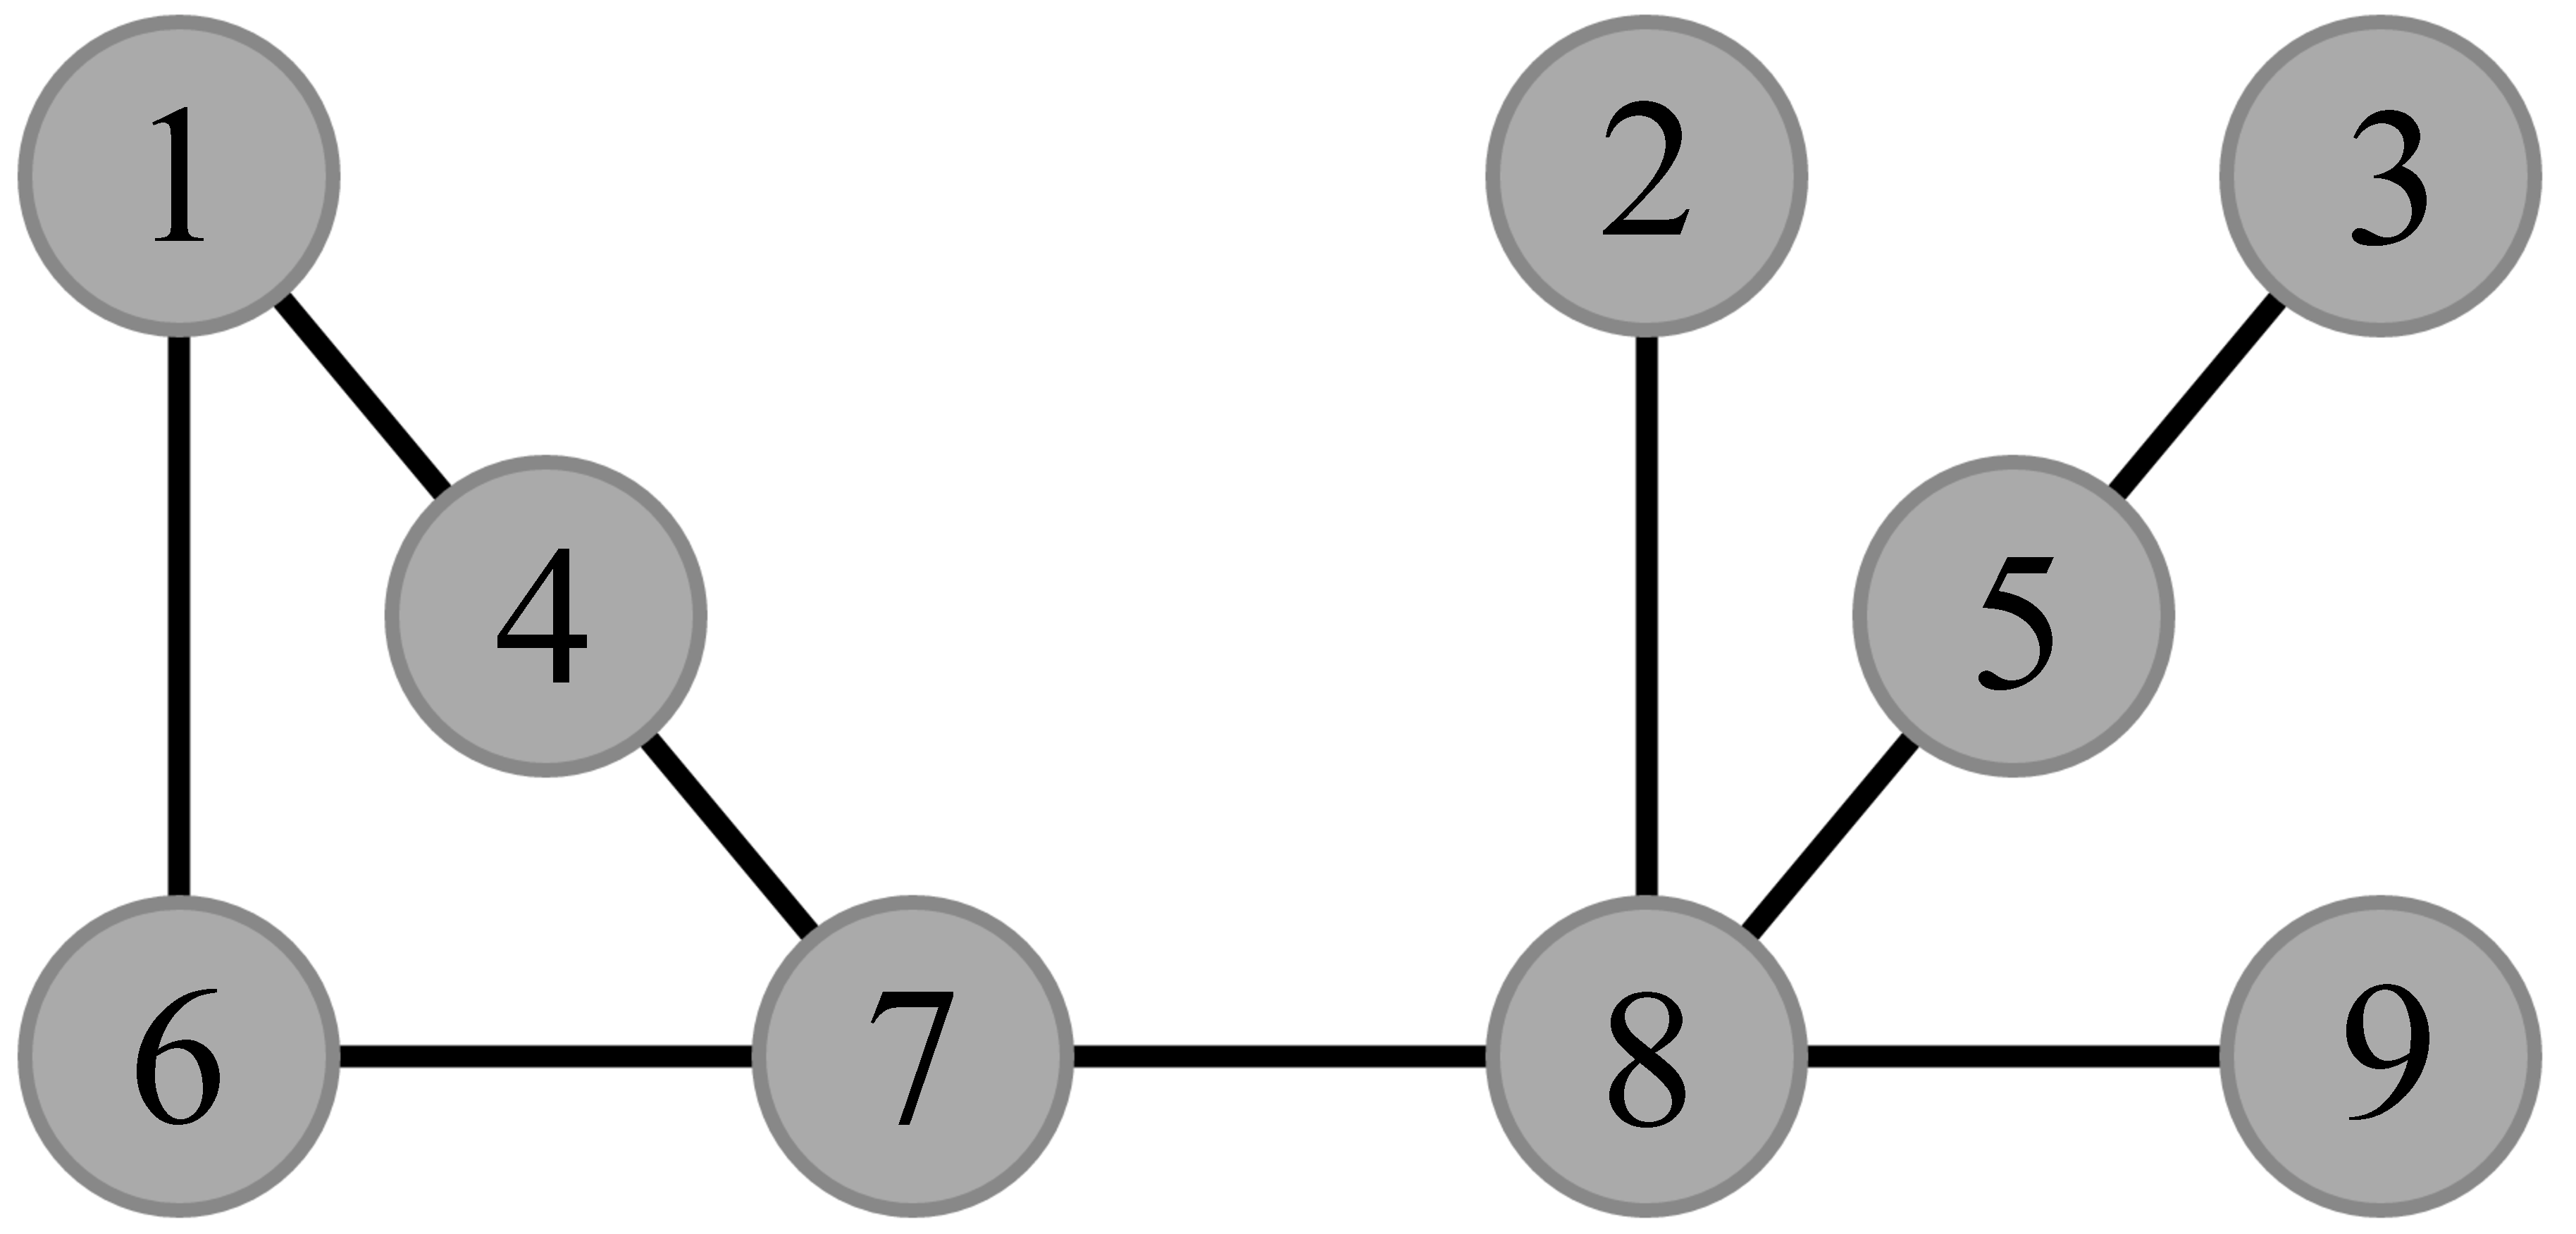
\includegraphics[width=6cm]{../figures/criterion.pdf}
         \caption{A simple, undirected graph $G$}
       \end{figure}
      }

      \only<2>{
        \vspace{0.25cm}
        \begin{columns}
          \begin{column}{0.5\textwidth}
            \begin{center}
              \begin{figure}
                 \centering
                 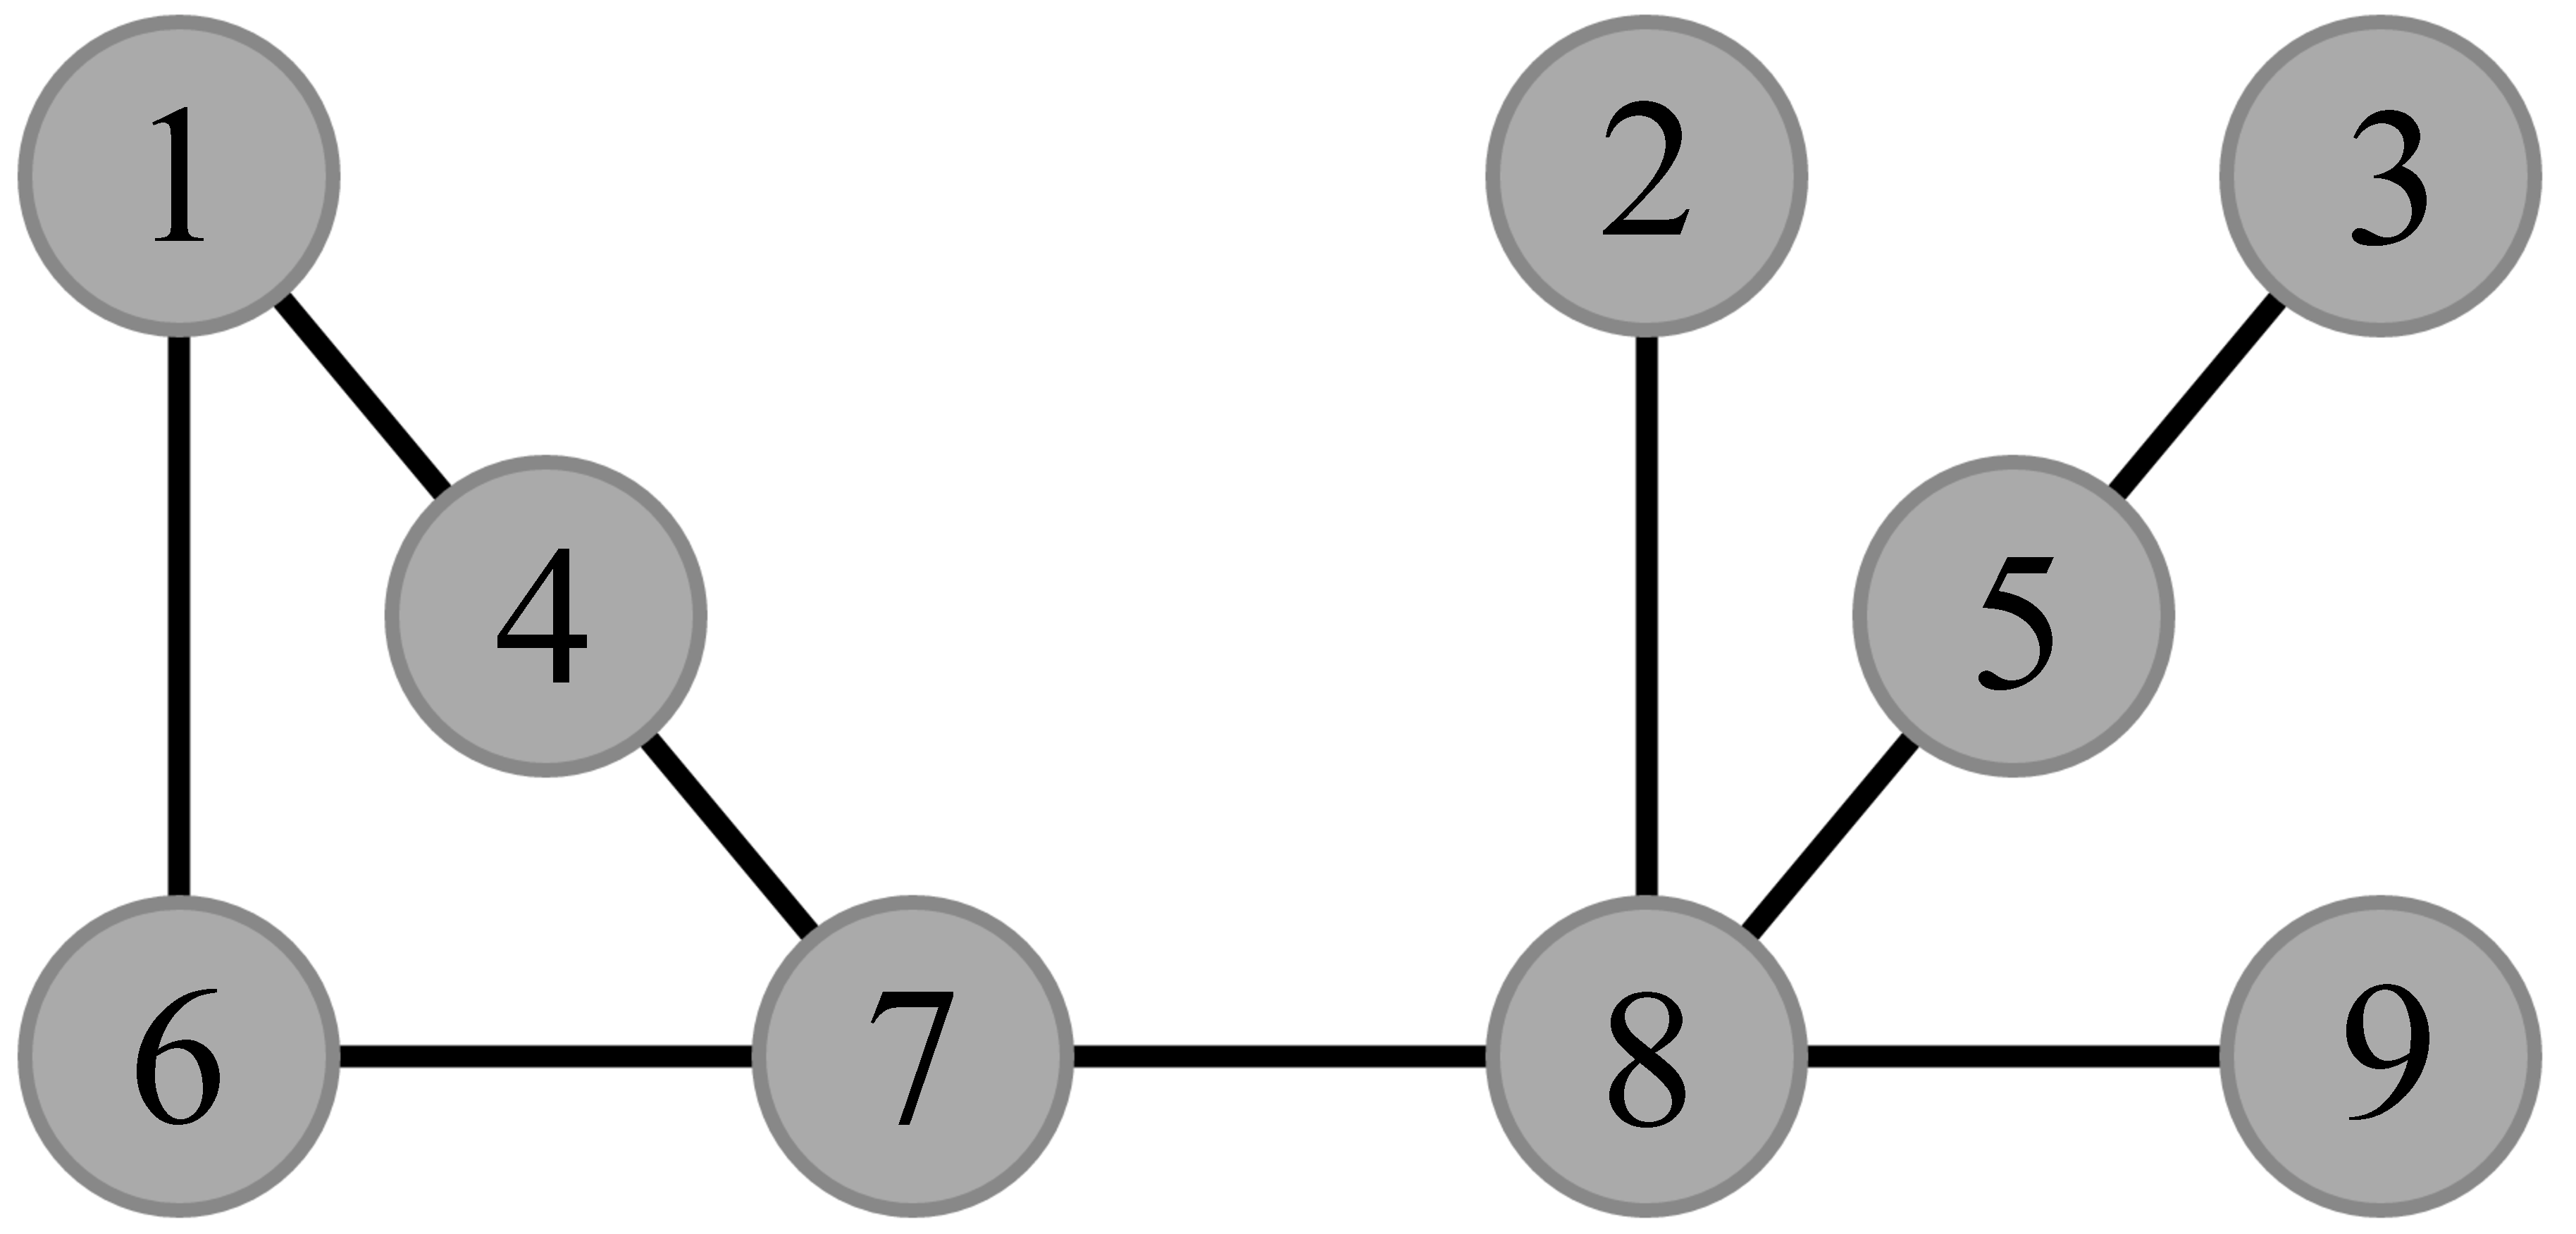
\includegraphics[width=6cm]{../figures/criterion.pdf}
                 \caption{A simple, undirected graph $G$}
               \end{figure}
            \end{center}
          \end{column}
          \begin{column}{0.5\textwidth}
            \begin{center}
              \begin{figure}
                \centering
                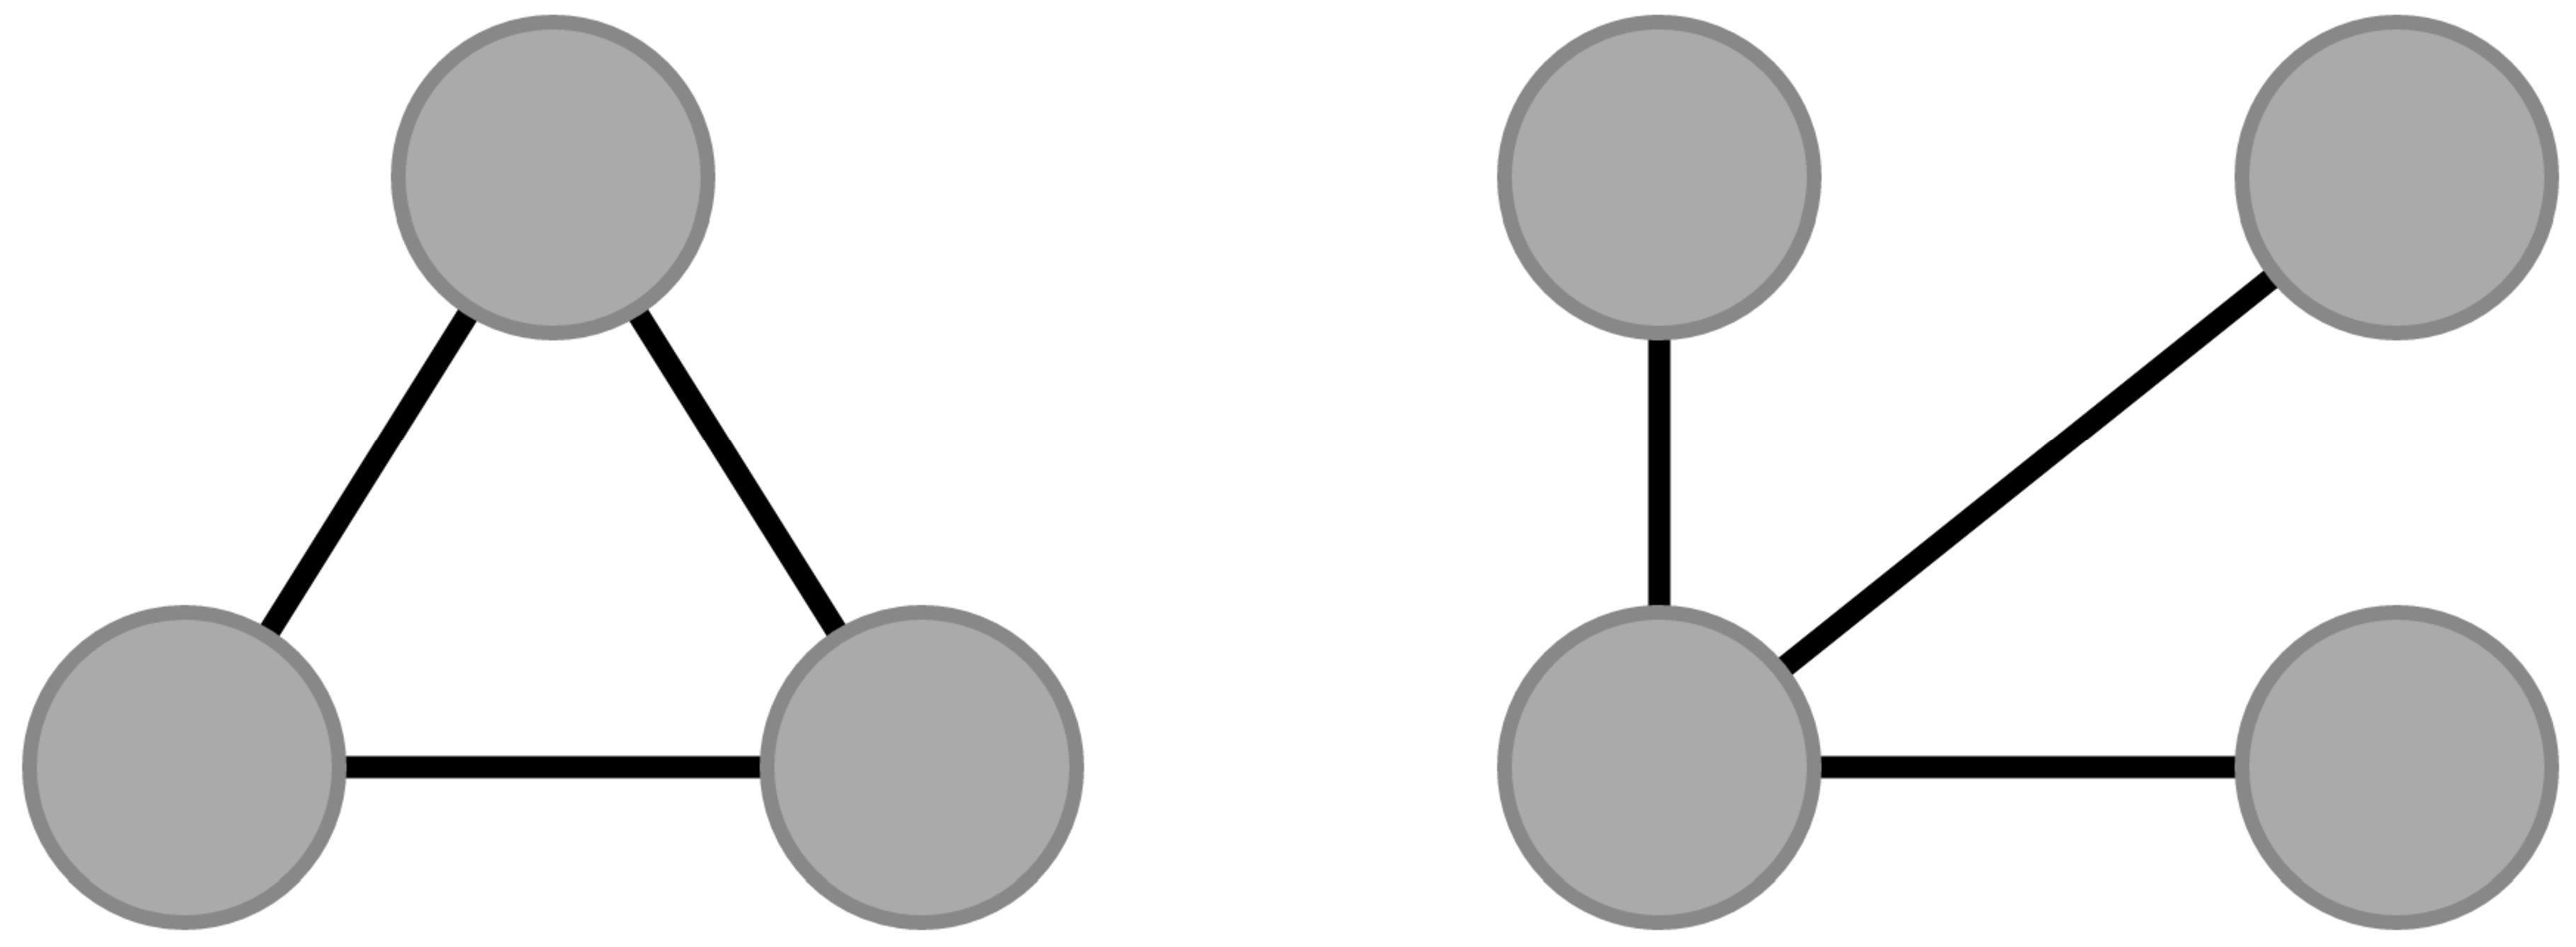
\includegraphics[width=6cm]{../figures/bad-criterion.pdf}
                \caption{Graphs $K_{3}$ and $K_{4}^{-3}$}
              \end{figure}
            \end{center}
          \end{column}
        \end{columns}
      }

      \only<3>{
        \vspace{0.25cm}
        \begin{columns}
          \begin{column}{0.5\textwidth}
            \begin{center}
              \begin{figure}
                 \centering
                 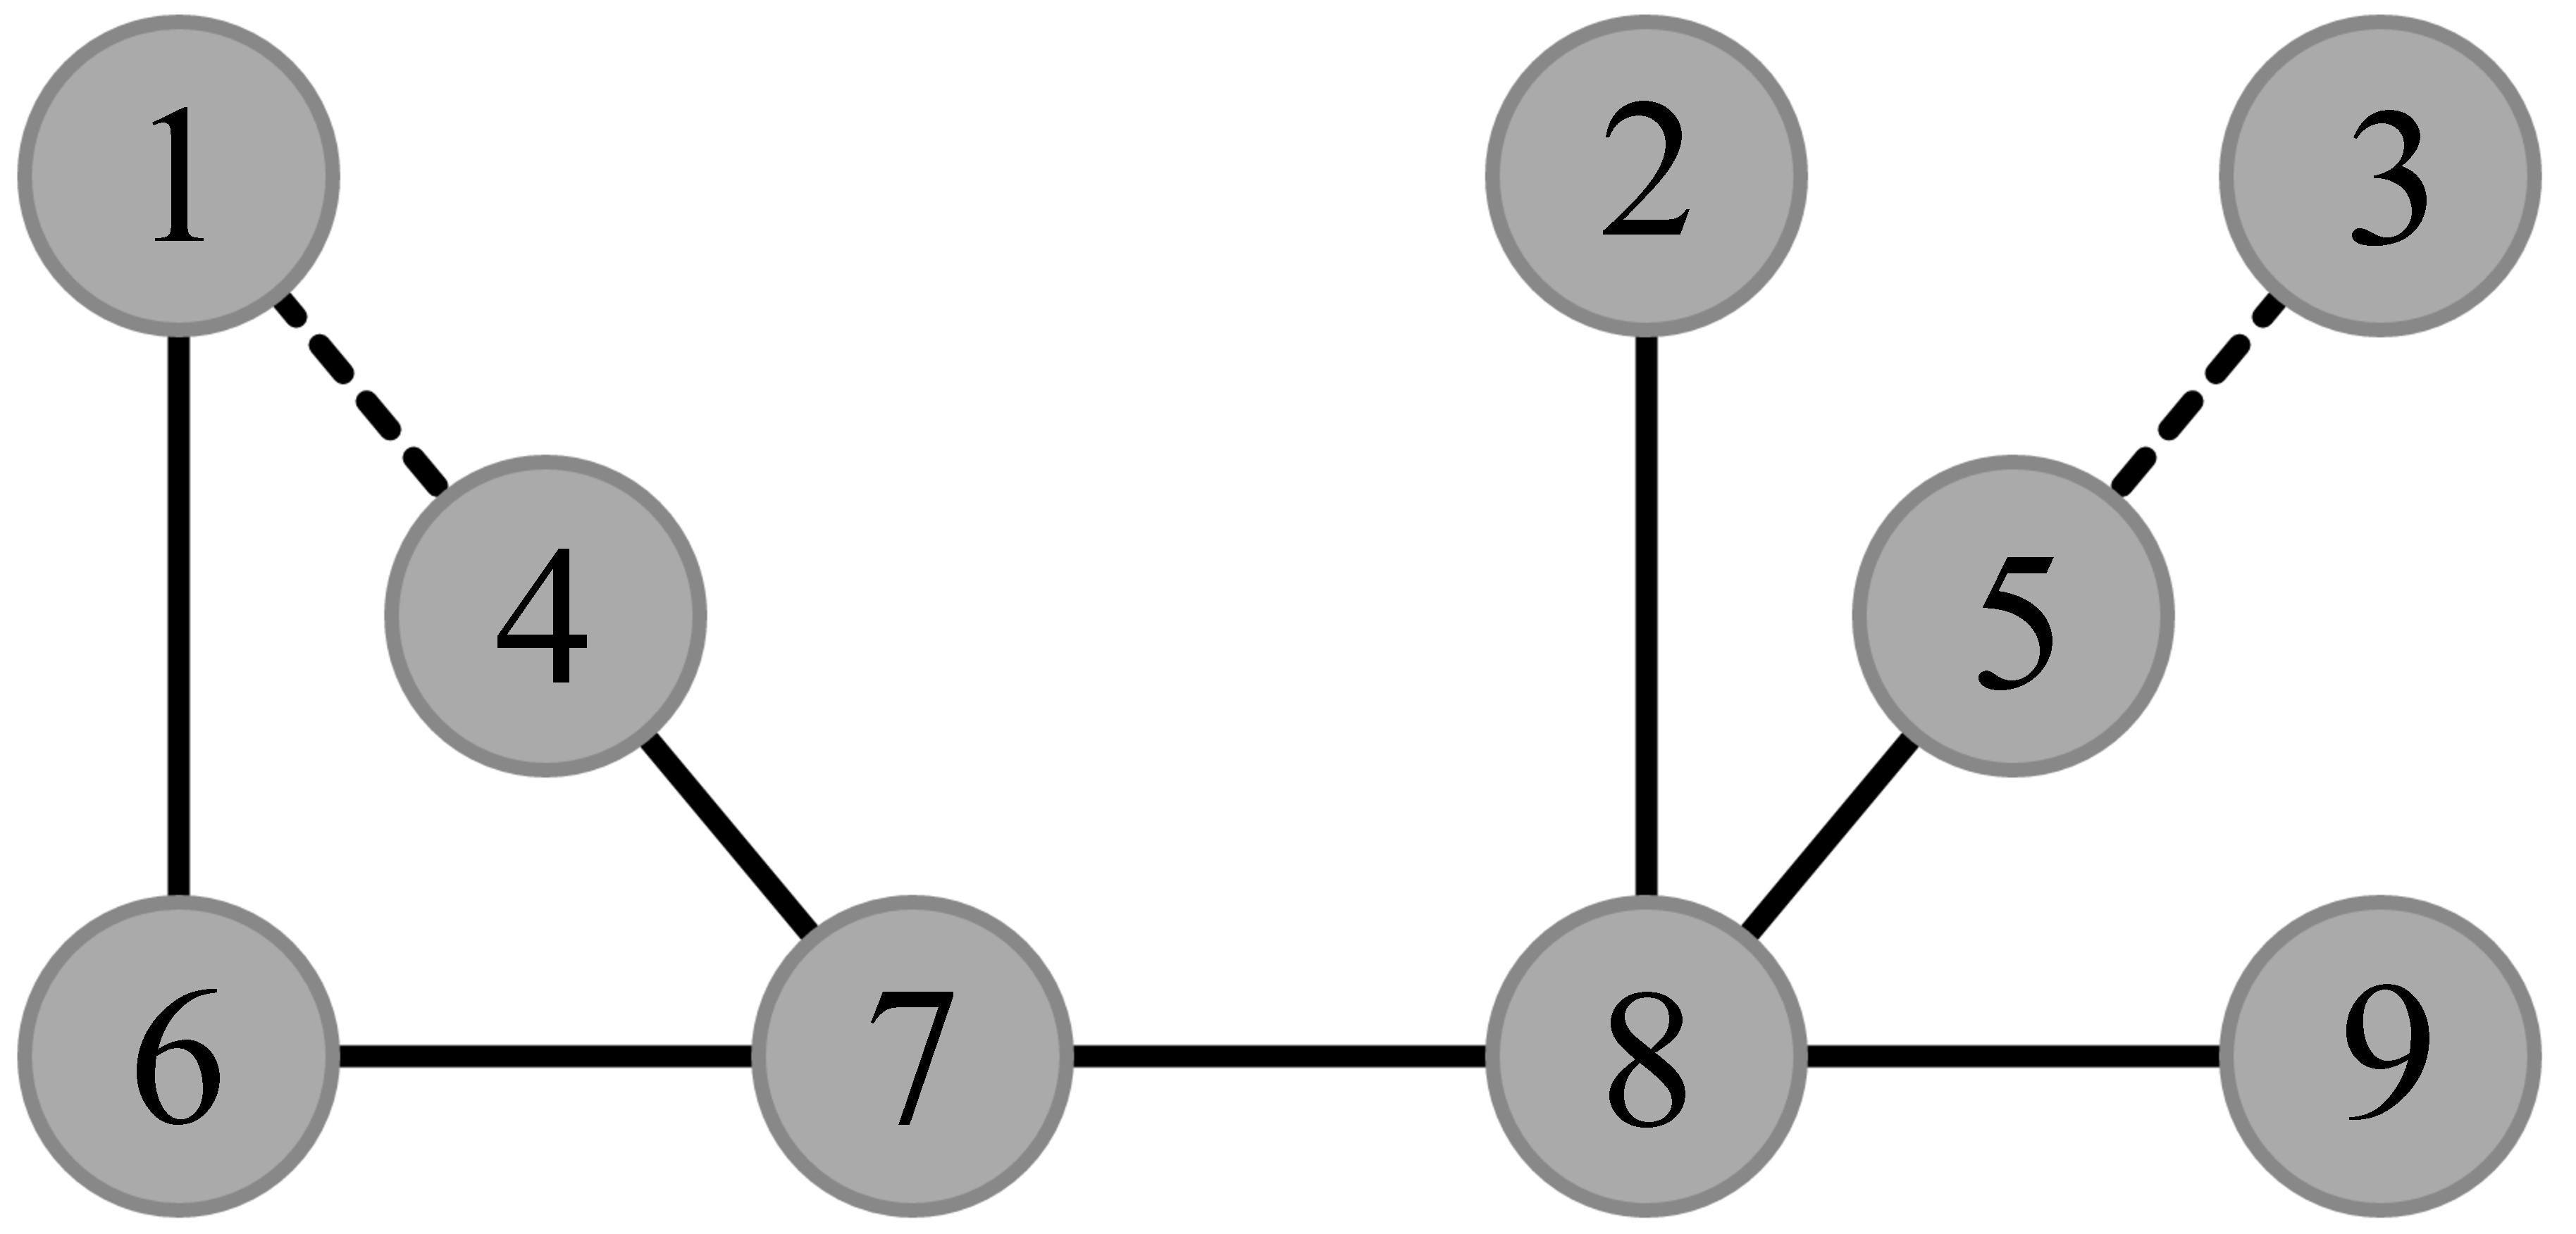
\includegraphics[width=6cm]{../figures/criterion-minor.pdf}
                 \caption{A simple, undirected graph $G$}
               \end{figure}
            \end{center}
          \end{column}
          \begin{column}{0.5\textwidth}
            \begin{center}
              \begin{figure}
                \centering
                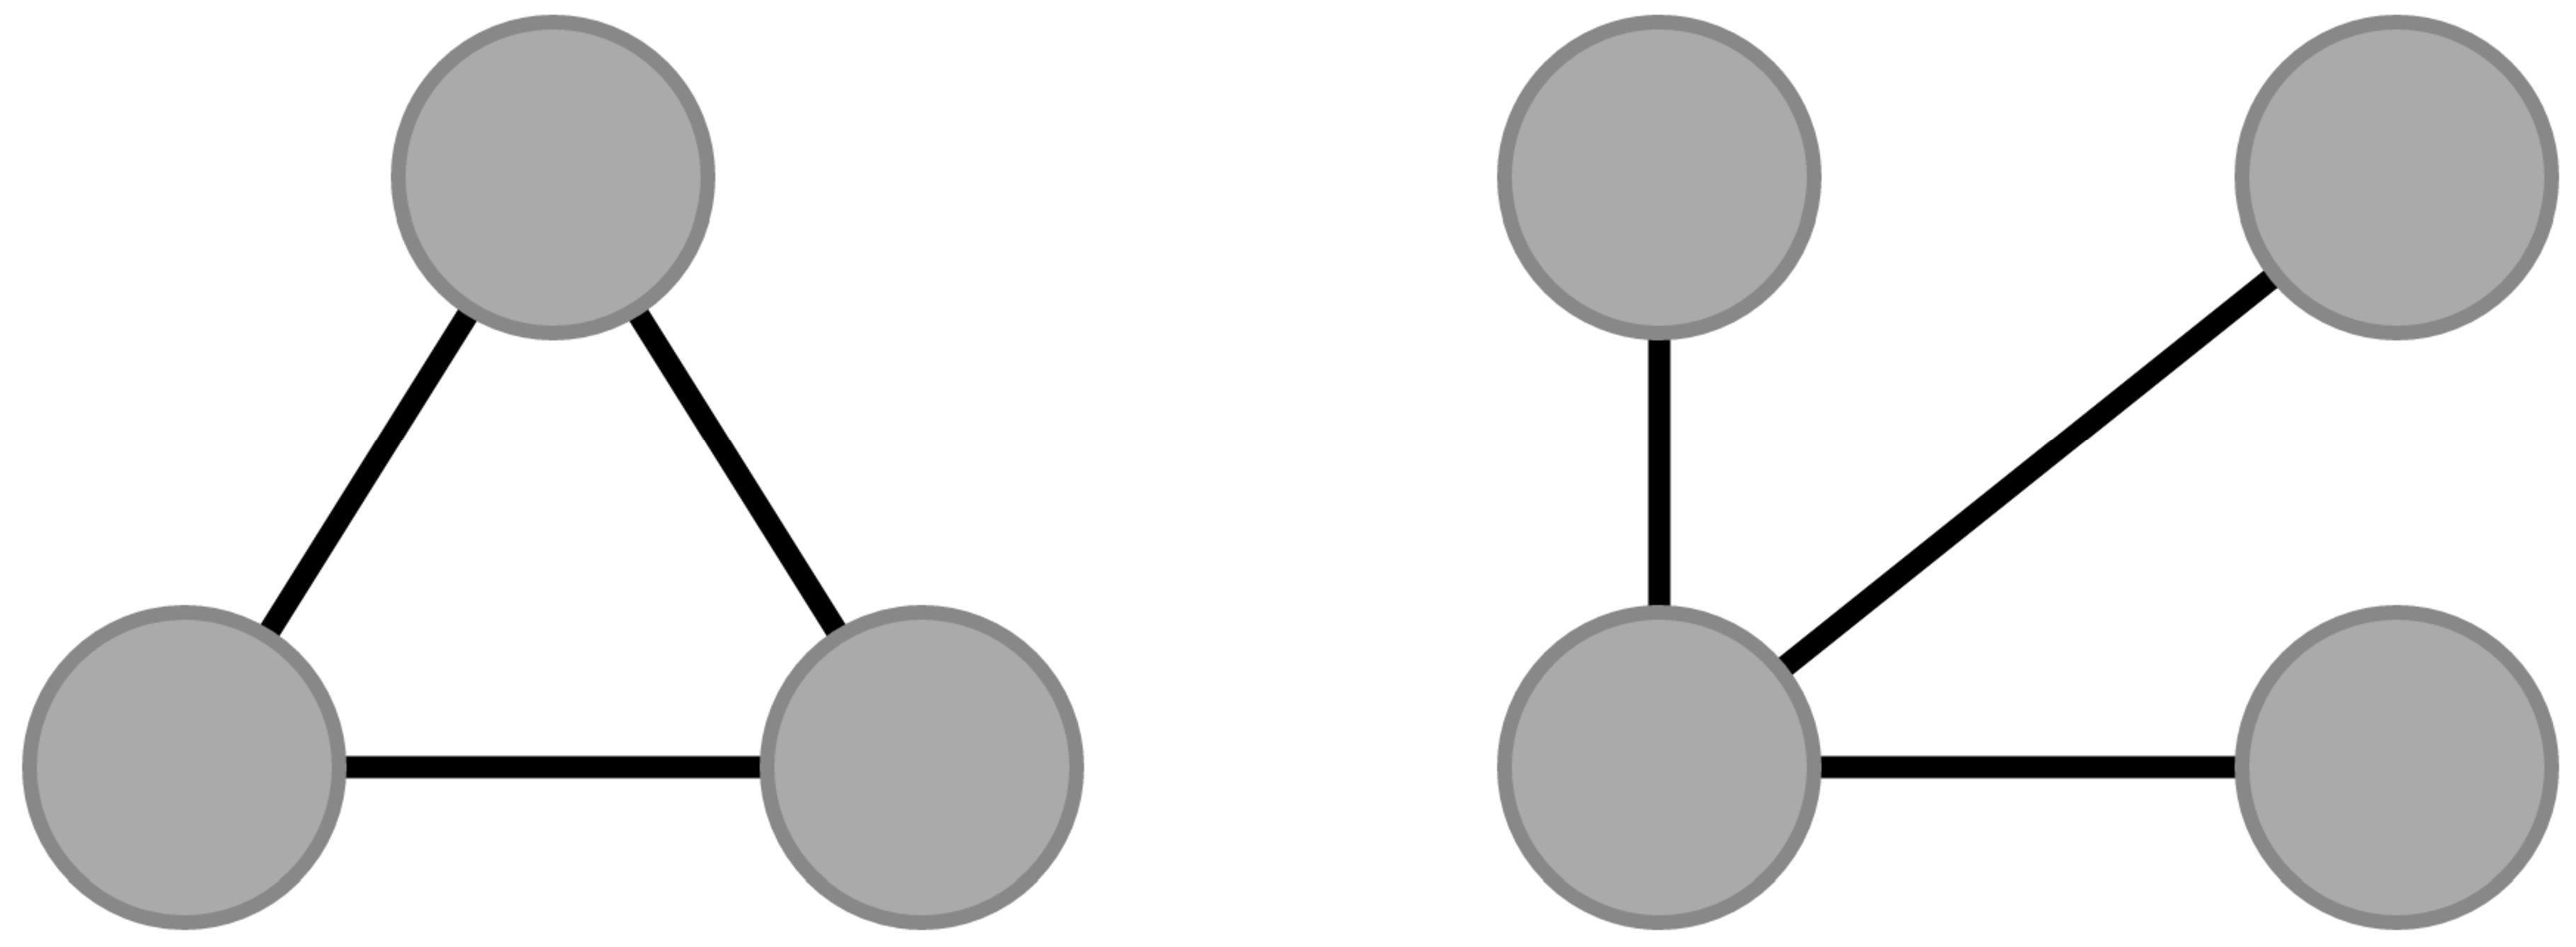
\includegraphics[width=6cm]{../figures/bad-criterion.pdf}
                \caption{Graphs $K_{3}$ and $K_{4}^{-3}$}
              \end{figure}
            \end{center}
          \end{column}
        \end{columns}
      }
    \end{textblock*}

    \begin{textblock*}{14cm}(1cm, 7.1cm) % {block width} (coords)
      To be conflict-free colored with 1 color, graph $G$ cannot contain $K_3$ or $K_4^{-3}$ as a minor. A graph is a \textbf{minor} if it can be formed by deleting and/or contracting edges from its parent graph. \only<3>{$G$ contains both $K_3$ and $K_4^{-3}$ as a minor and thus {\color{red}\textbf{cannot}} be conflict-free colored with 1 color.}
    \end{textblock*}

  \end{frame}

  \begin{frame}
    \frametitle{Iterated Elimination of Distance-3-Sets}

    \only<1>{
      \begin{columns}
        \begin{column}{0.5\textwidth}
          \begin{algorithm}[H]
            \caption*{\textbf{Algorithm} IEDS}
            \scriptsize
            \begin{algorithmic}[1]
            \State $i \gets 1$
            \State Remove all isolated paths from $G$
            \While{$G$ is not empty}
              \State $D \gets \emptyset$
              \ForAll{components of $G$}
                \State Pick any vertex $v$
                \State $D \gets D \cup \{ v \}$
                \While{$\exists u$ at distance $\geq 3$ $\forall v \in D$}
                  \State Pick $u$ at distance 3 from some vertex in $D$
                  \State $D \gets D \cup \{ w \}$
                \EndWhile
                \ForAll{$u \in D$}
                  \State Color $u$ with color $i$
                \EndFor
                \State $i \gets i + 1$
                \ForAll{$u \in D$}
                  \State Remove $N(u)$ from $G$
                \EndFor
                \State Remove all isolated paths from G
              \EndFor
            \EndWhile
            \State Color all removed isolated paths using color $i$
            \end{algorithmic}
          \end{algorithm}
        \end{column}
        \begin{column}{0.5\textwidth}
          \begin{center}
            \begin{textblock*}{8cm}(8cm, 2cm) % {block width} (coords)
              \begin{figure}
                \centering
                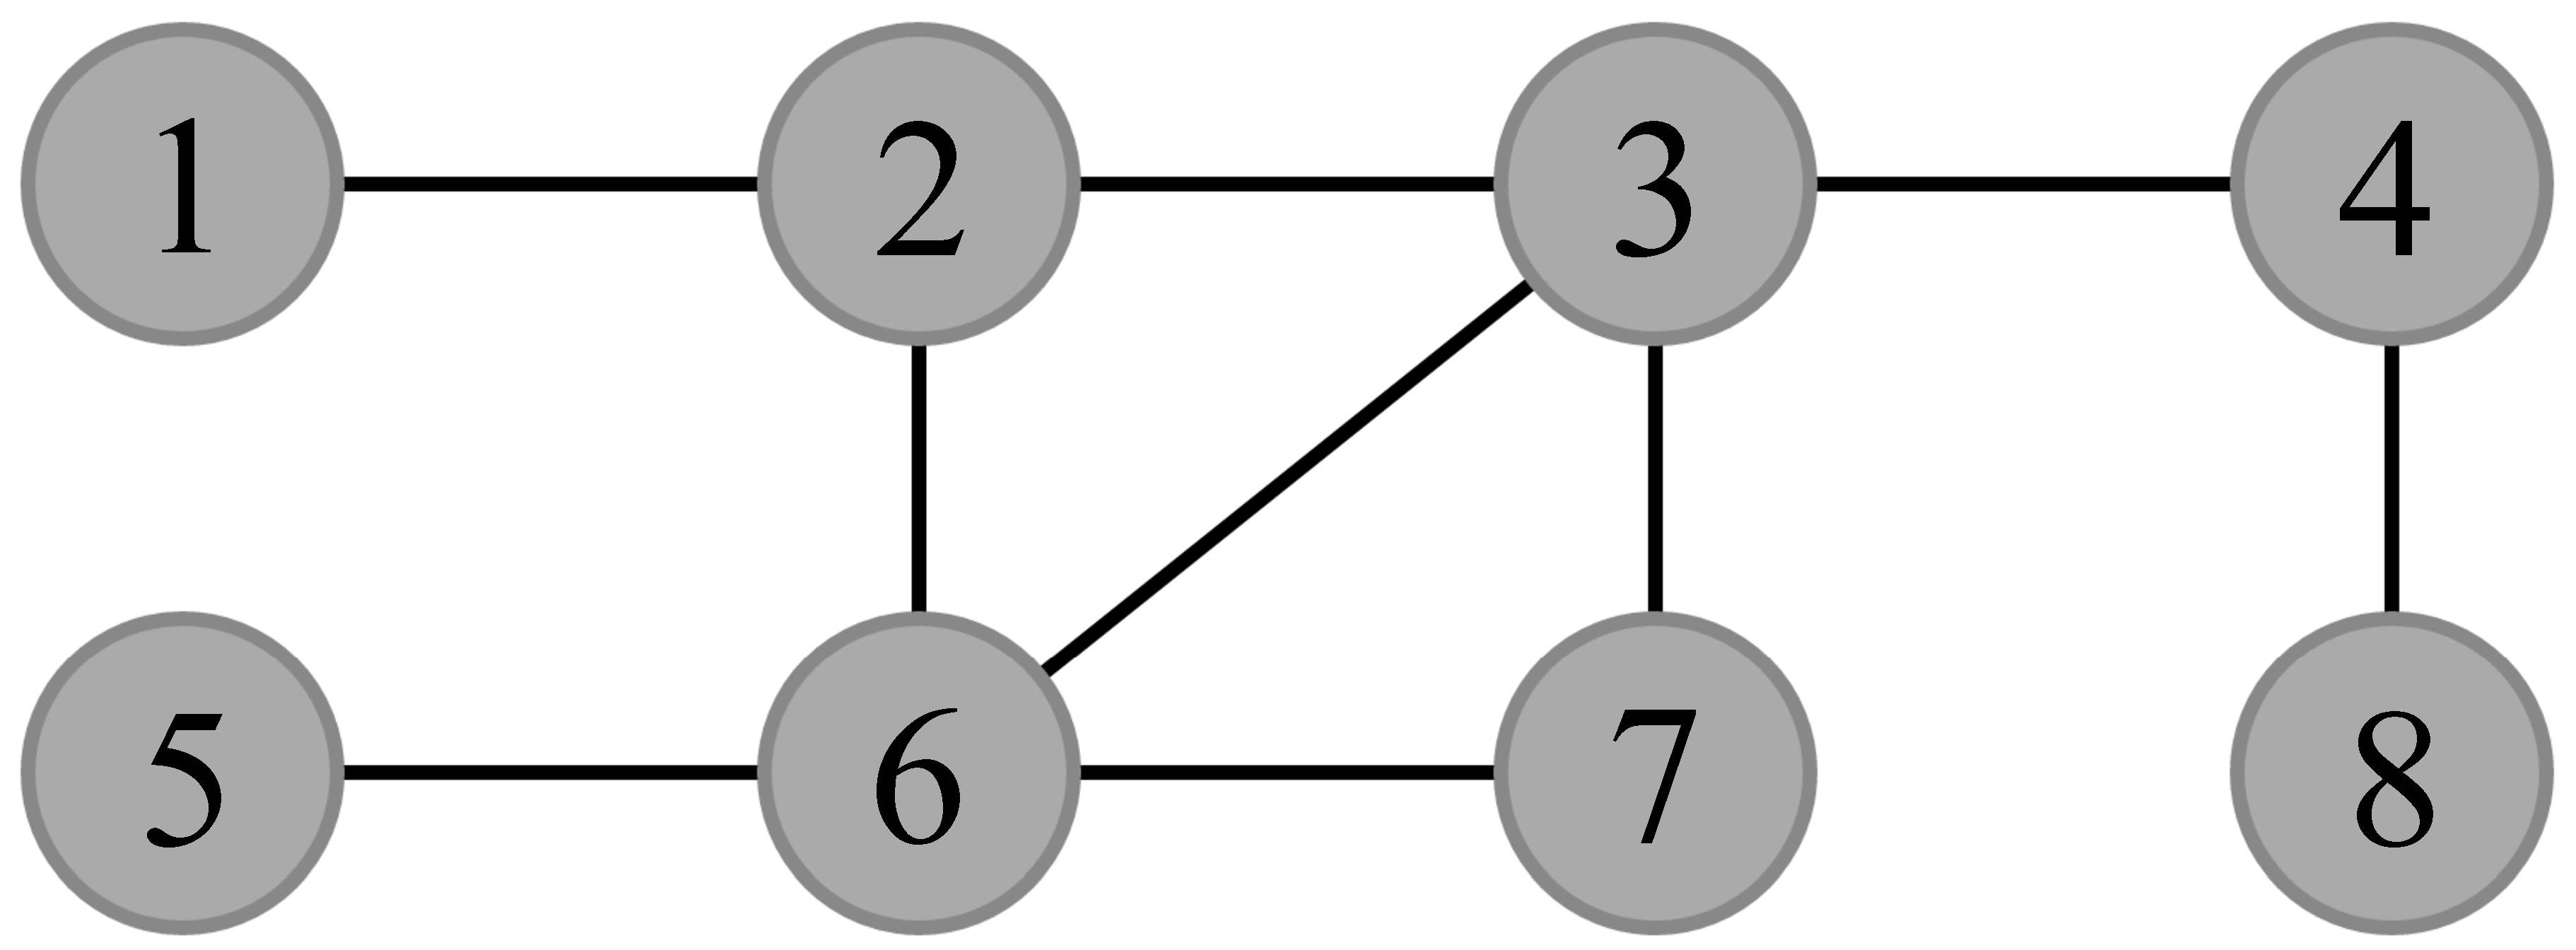
\includegraphics[width=6cm]{../figures/algorithm1.pdf}
                \caption*{A simple, undirected graph $G$}
              \end{figure}
            \end{textblock*}
          \end{center}
        \end{column}
      \end{columns}
    }

    \only<2-6>{
      \begin{textblock*}{8cm}(8cm, 6cm) % {block width} (coords)
        \begin{center}
          $i= 1$
        \end{center}
      \end{textblock*}
    }

    \only<2>{
      \begin{columns}
        \begin{column}{0.5\textwidth}
          \begin{algorithm}[H]
            \caption*{\textbf{Algorithm} IEDS}
            \scriptsize
            \begin{algorithmic}[1]
            \State \algemph{$i \gets 1$}
            \State \algemph{Remove all isolated paths from $G$}
            \While{$G$ is not empty}
              \State $D \gets \emptyset$
              \ForAll{components of $G$}
                \State Pick any vertex $v$
                \State $D \gets D \cup \{ v \}$
                \While{$\exists u$ at distance $\geq 3$ $\forall v \in D$}
                  \State Pick $u$ at distance 3 from some vertex in $D$
                  \State $D \gets D \cup \{ w \}$
                \EndWhile
                \ForAll{$u \in D$}
                  \State Color $u$ with color $i$
                \EndFor
                \State $i \gets i + 1$
                \ForAll{$u \in D$}
                  \State Remove $N(u)$ from $G$
                \EndFor
                \State Remove all isolated paths from G
              \EndFor
            \EndWhile
            \State Color all removed isolated paths using color $i$
            \end{algorithmic}
          \end{algorithm}
        \end{column}
        \begin{column}{0.5\textwidth}
          \begin{center}
            \begin{textblock*}{8cm}(8cm, 2cm) % {block width} (coords)
              \begin{figure}
                \centering
                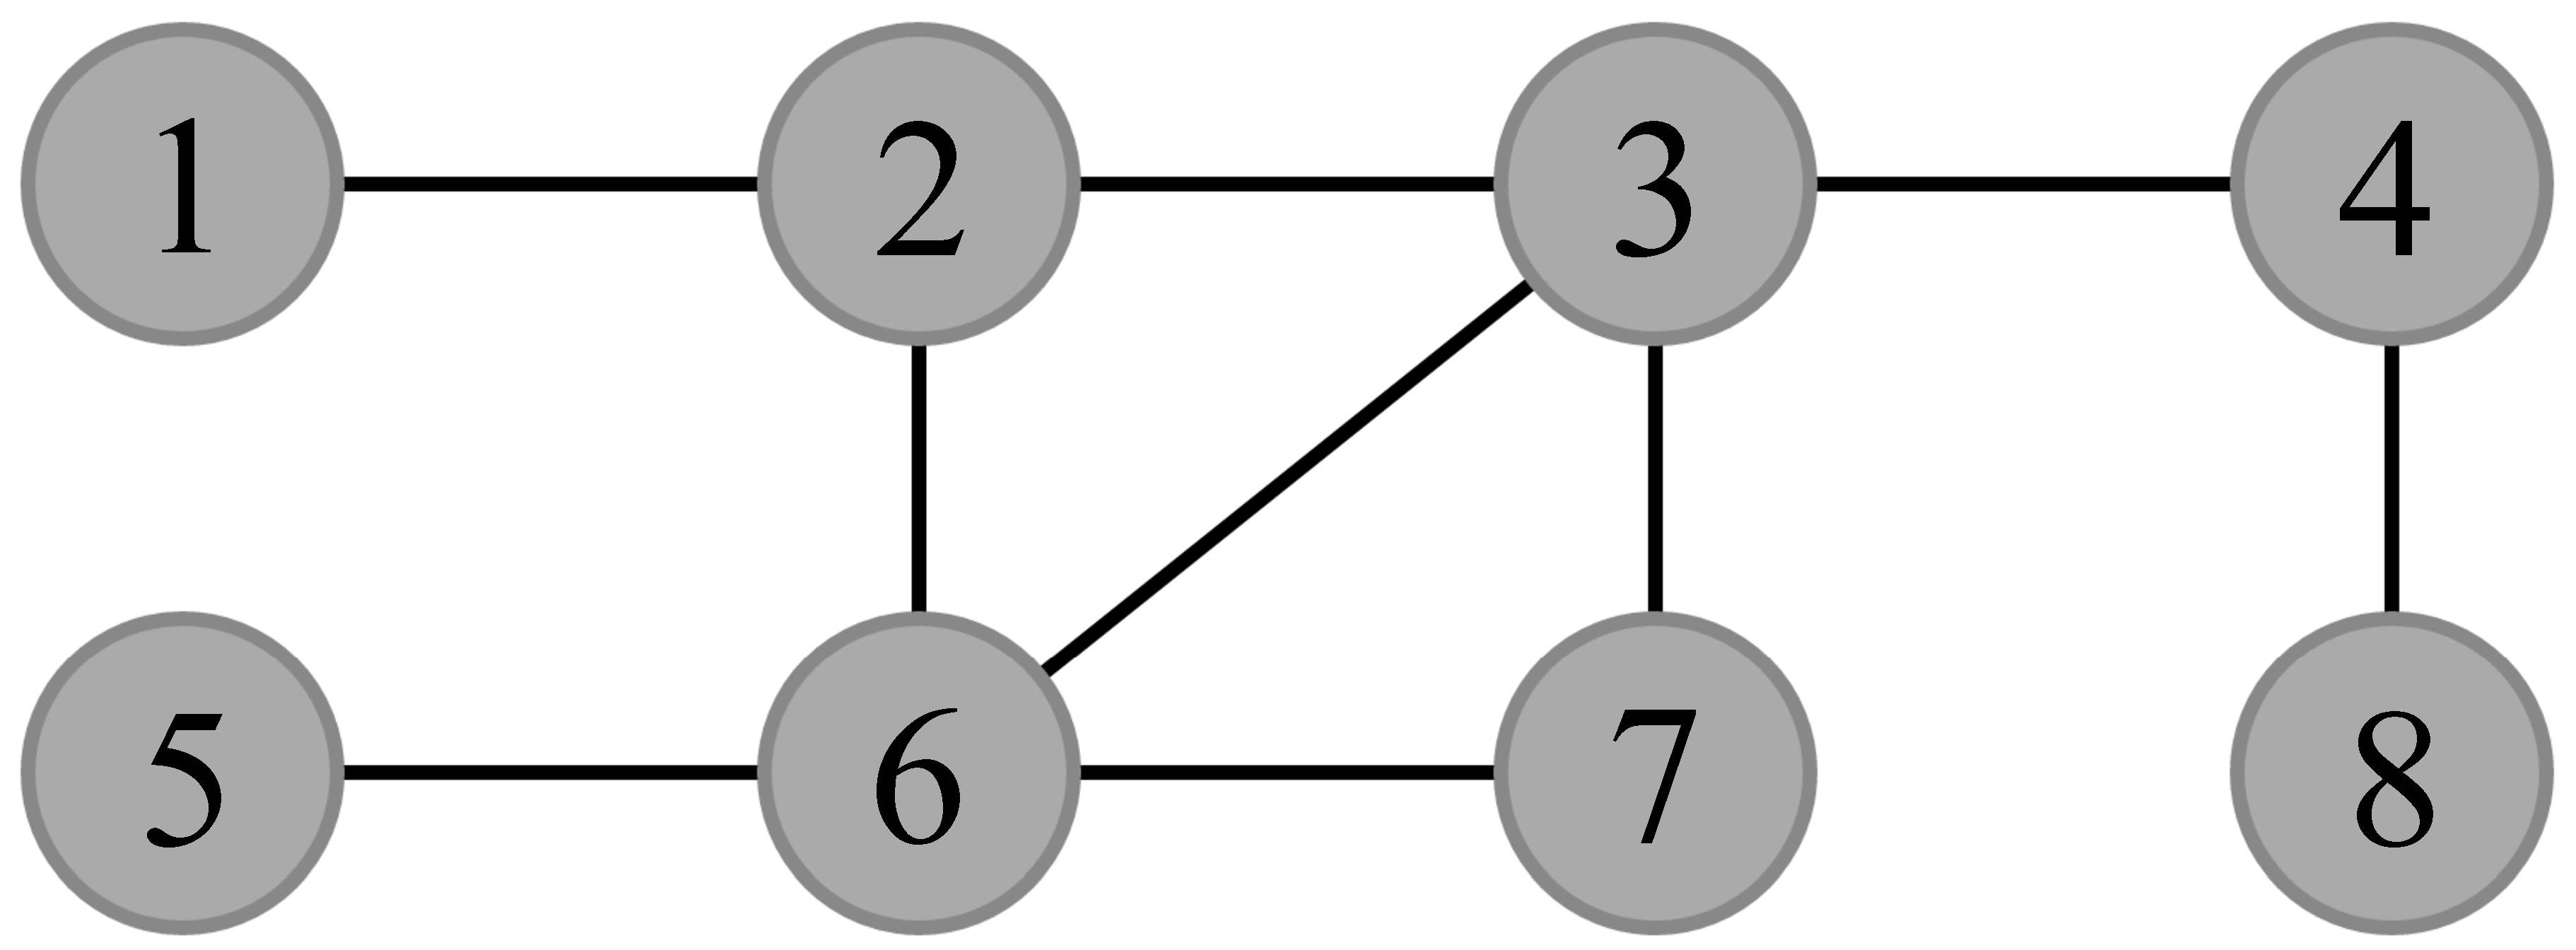
\includegraphics[width=6cm]{../figures/algorithm1.pdf}
                \caption*{A simple, undirected graph $G$}
              \end{figure}
            \end{textblock*}
          \end{center}
        \end{column}
      \end{columns}
    }

    \only<3>{
      \begin{textblock*}{8cm}(8cm, 6.5cm) % {block width} (coords)
        \begin{center}
          $D= \{\}$
        \end{center}
      \end{textblock*}

      \begin{columns}
        \begin{column}{0.5\textwidth}
          \begin{algorithm}[H]
            \caption*{\textbf{Algorithm} IEDS}
            \scriptsize
            \begin{algorithmic}[1]
            \State $i \gets 1$
            \State Remove all isolated paths from $G$
            \While{$G$ is not empty}
              \State \algemph{$D \gets \emptyset$}
              \ForAll{components of $G$}
                \State Pick any vertex $v$
                \State $D \gets D \cup \{ v \}$
                \While{$\exists u$ at distance $\geq 3$ $\forall v \in D$}
                  \State Pick $u$ at distance 3 from some vertex in $D$
                  \State $D \gets D \cup \{ w \}$
                \EndWhile
                \ForAll{$u \in D$}
                  \State Color $u$ with color $i$
                \EndFor
                \State $i \gets i + 1$
                \ForAll{$u \in D$}
                  \State Remove $N(u)$ from $G$
                \EndFor
                \State Remove all isolated paths from G
              \EndFor
            \EndWhile
            \State Color all removed isolated paths using color $i$
            \end{algorithmic}
          \end{algorithm}
        \end{column}
        \begin{column}{0.5\textwidth}
          \begin{center}
            \begin{textblock*}{8cm}(8cm, 2cm) % {block width} (coords)
              \begin{figure}
                \centering
                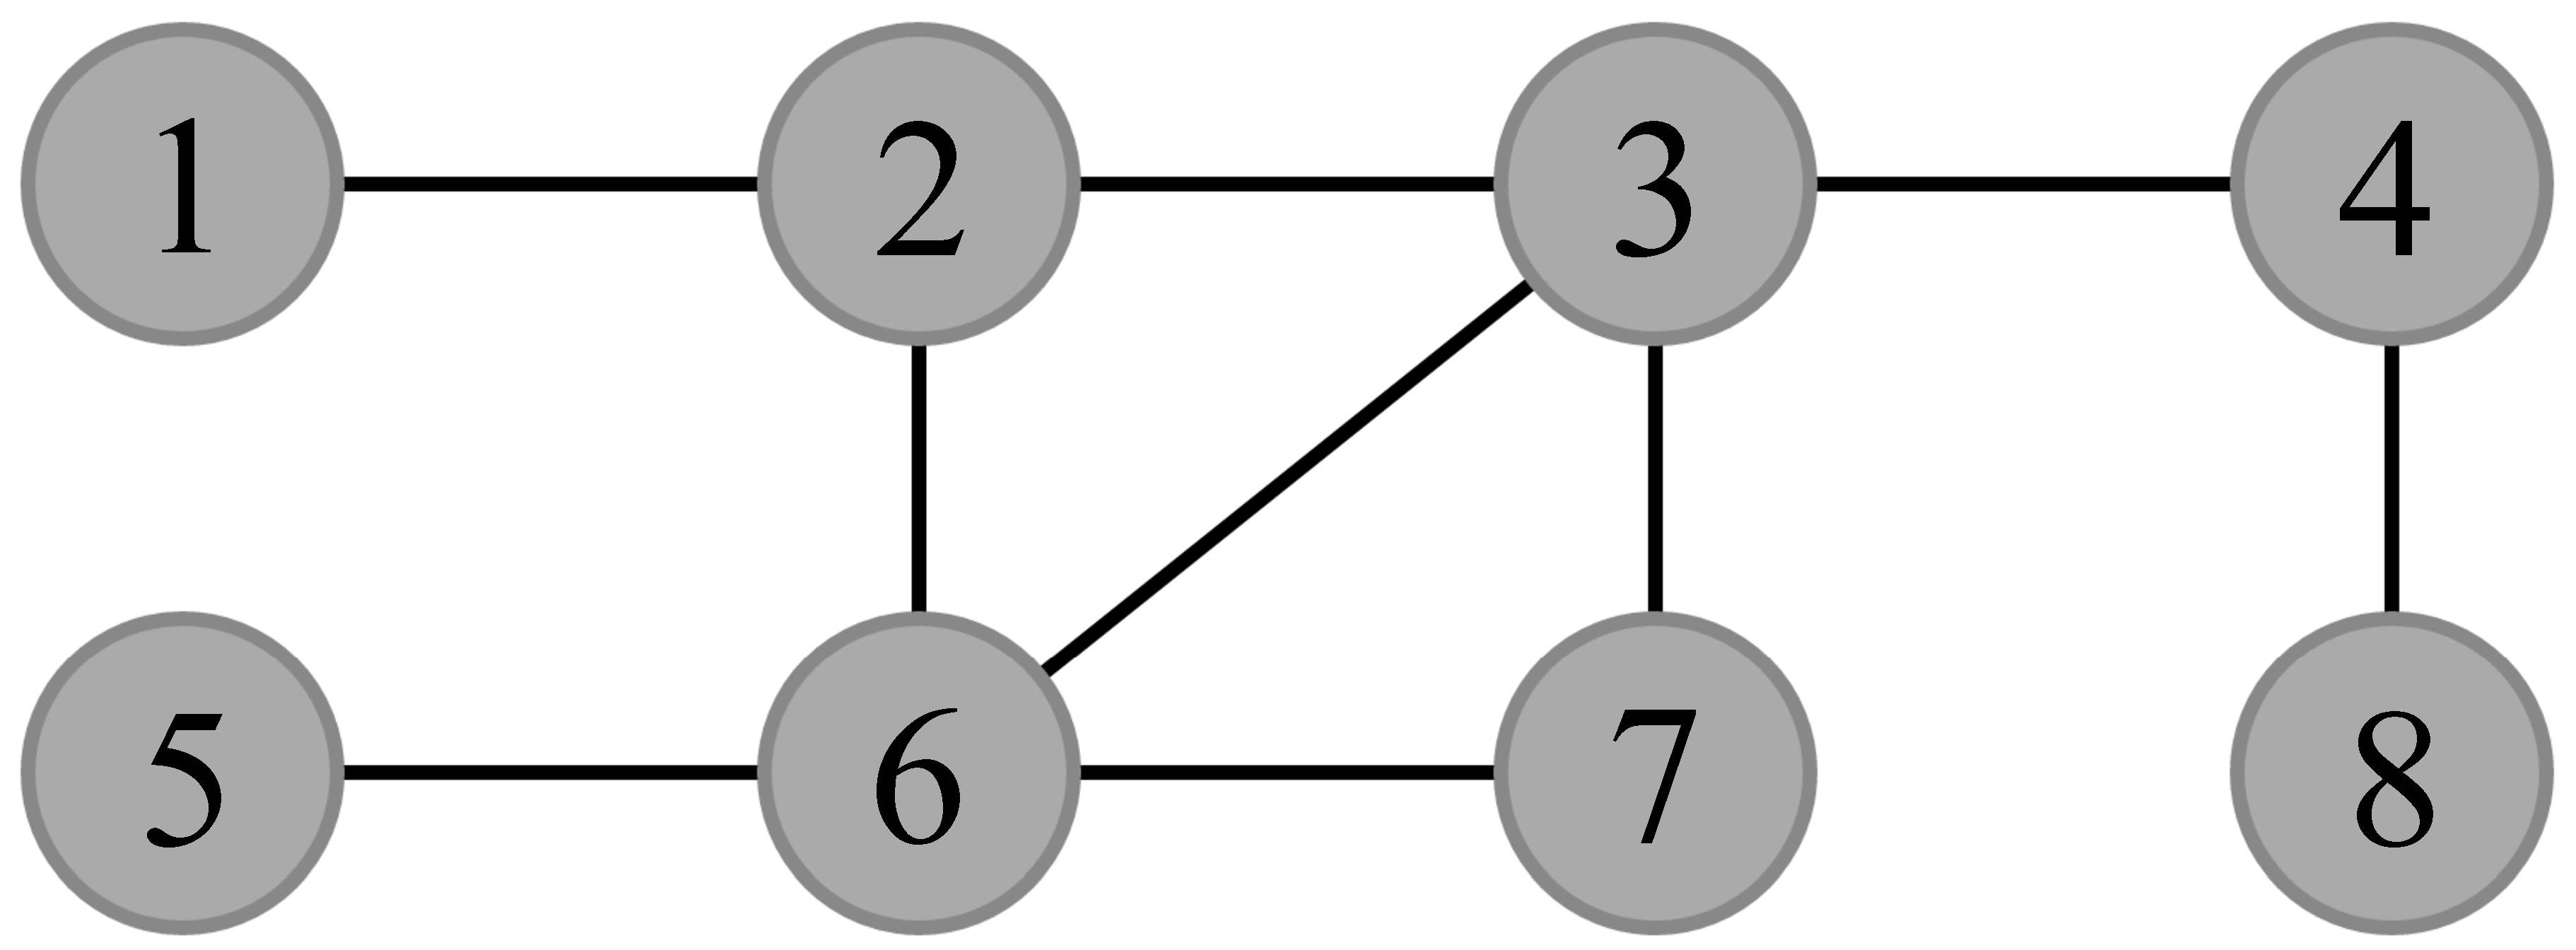
\includegraphics[width=6cm]{../figures/algorithm1.pdf}
                \caption*{A simple, undirected graph $G$}
              \end{figure}
            \end{textblock*}
          \end{center}
        \end{column}
      \end{columns}
    }

    \only<4>{
      \begin{textblock*}{8cm}(8cm, 6.5cm) % {block width} (coords)
        \begin{center}
          $D= \{8\}$
        \end{center}
      \end{textblock*}

      \begin{columns}
        \begin{column}{0.5\textwidth}
          \begin{algorithm}[H]
            \caption*{\textbf{Algorithm} IEDS}
            \scriptsize
            \begin{algorithmic}[1]
            \State $i \gets 1$
            \State Remove all isolated paths from $G$
            \While{$G$ is not empty}
              \State $D \gets \emptyset$
              \ForAll{components of $G$}
                \State \algemph{Pick any vertex $v$}
                \State \algemph{$D \gets D \cup \{ v \}$}
                \While{$\exists u$ at distance $\geq 3$ $\forall v \in D$}
                  \State Pick $u$ at distance 3 from some vertex in $D$
                  \State $D \gets D \cup \{ w \}$
                \EndWhile
                \ForAll{$u \in D$}
                  \State Color $u$ with color $i$
                \EndFor
                \State $i \gets i + 1$
                \ForAll{$u \in D$}
                  \State Remove $N(u)$ from $G$
                \EndFor
                \State Remove all isolated paths from G
              \EndFor
            \EndWhile
            \State Color all removed isolated paths using color $i$
            \end{algorithmic}
          \end{algorithm}
        \end{column}
        \begin{column}{0.5\textwidth}
          \begin{center}
            \begin{textblock*}{8cm}(8cm, 2cm) % {block width} (coords)
              \begin{figure}
                \centering
                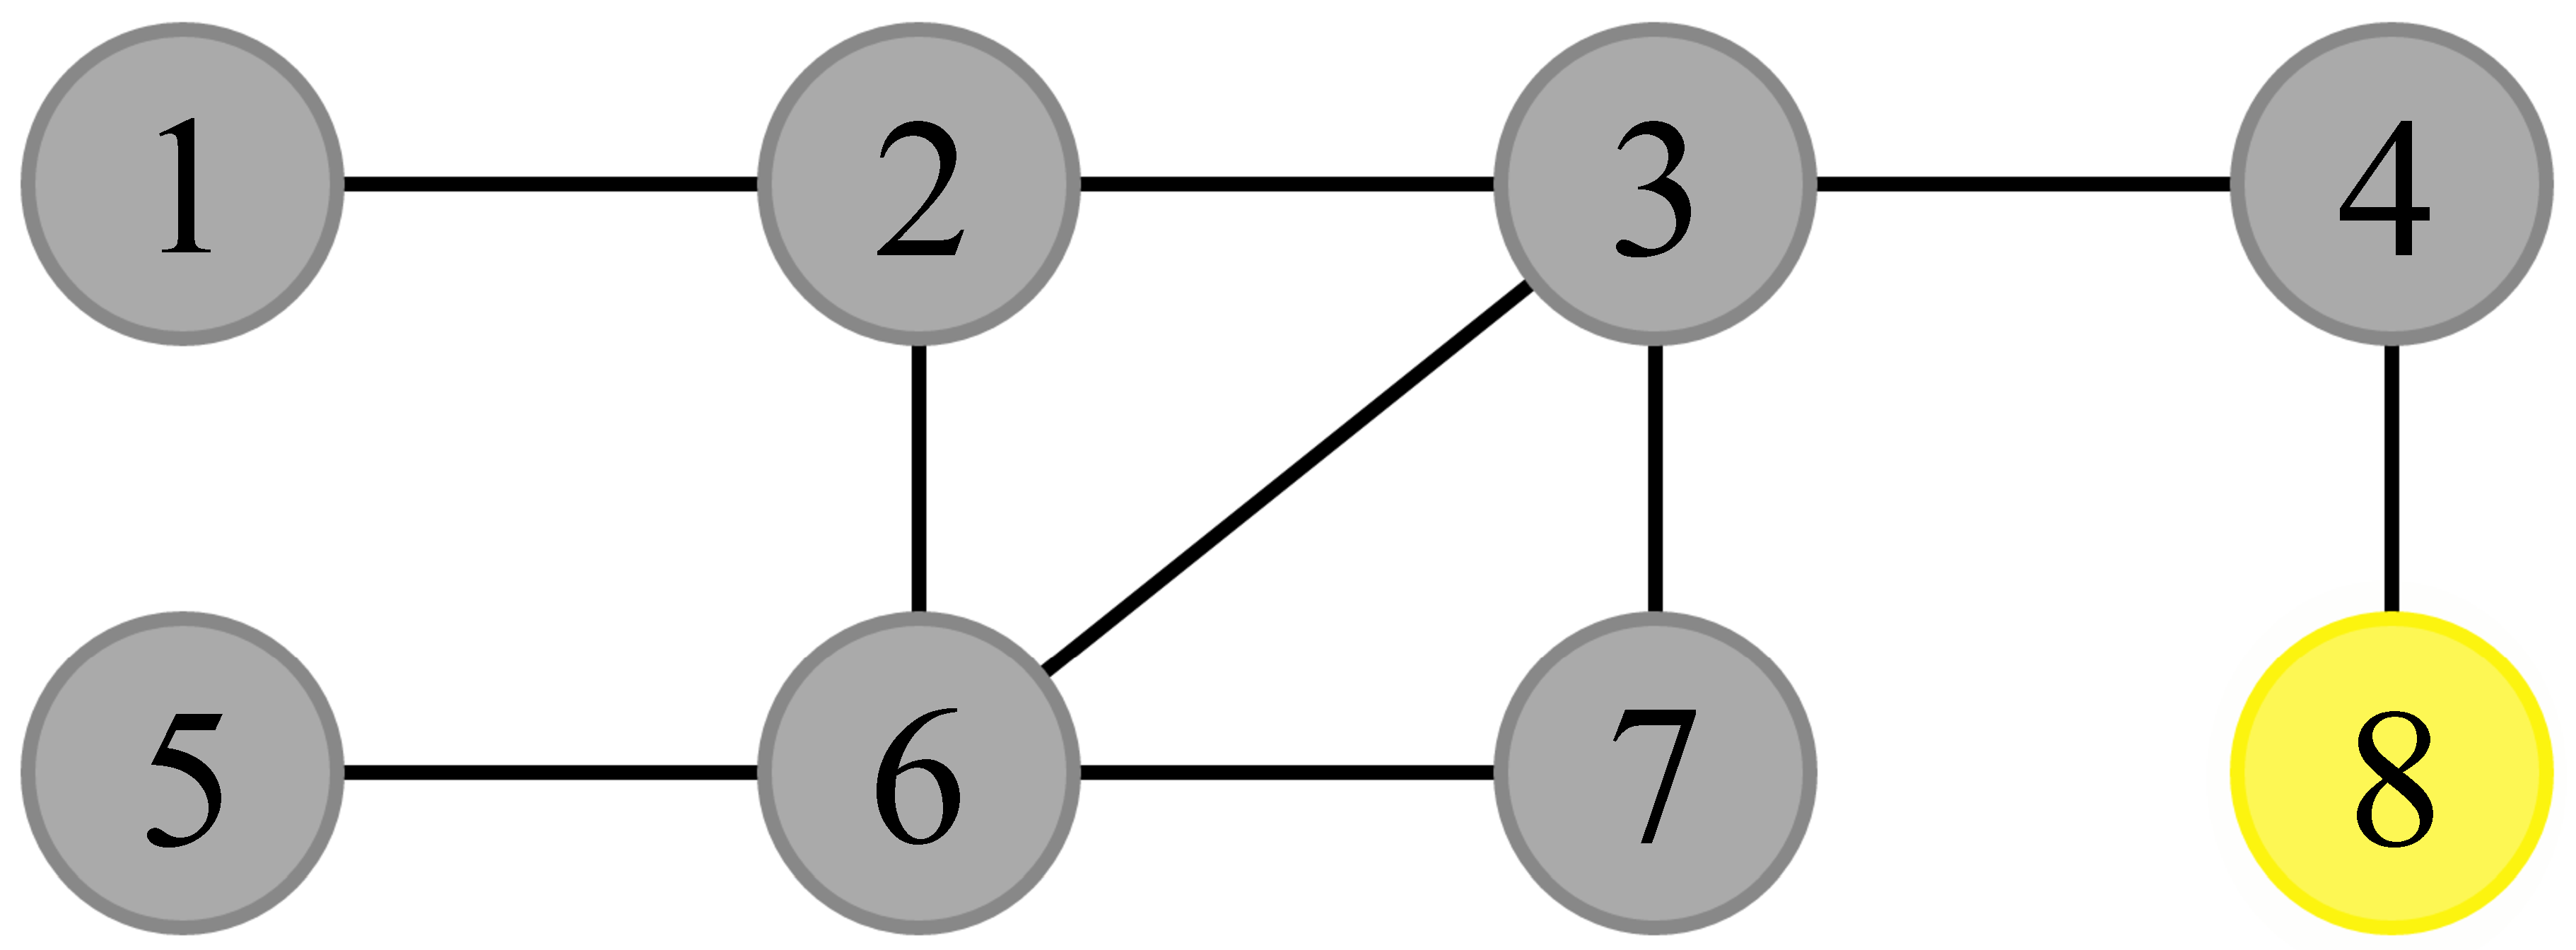
\includegraphics[width=6cm]{../figures/algorithm1-slide-1.pdf}
                \caption*{A simple, undirected graph $G$}
              \end{figure}
            \end{textblock*}
          \end{center}
        \end{column}
      \end{columns}
    }

    \only<5>{
      \begin{textblock*}{8cm}(8cm, 6.5cm) % {block width} (coords)
        \begin{center}
          $D= \{8\}$
        \end{center}
      \end{textblock*}

      \begin{columns}
        \begin{column}{0.5\textwidth}
          \begin{algorithm}[H]
            \caption*{\textbf{Algorithm} IEDS}
            \scriptsize
            \begin{algorithmic}[1]
            \State $i \gets 1$
            \State Remove all isolated paths from $G$
            \While{$G$ is not empty}
              \State $D \gets \emptyset$
              \ForAll{components of $G$}
                \State Pick any vertex $v$}
                \State $D \gets D \cup \{ v \}$
                \While{$\exists u$ at distance $\geq 3$ $\forall v \in D$}
                  \State Pick $u$ at distance 3 from some vertex in $D$
                  \State $D \gets D \cup \{ w \}$
                \EndWhile
                \ForAll{$u \in D$}
                  \State Color $u$ with color $i$
                \EndFor
                \State $i \gets i + 1$
                \ForAll{$u \in D$}
                  \State Remove $N(u)$ from $G$
                \EndFor
                \State Remove all isolated paths from G
              \EndFor
            \EndWhile
            \State Color all removed isolated paths using color $i$
            \end{algorithmic}
          \end{algorithm}
        \end{column}
        \begin{column}{0.5\textwidth}
          \begin{center}
            \begin{textblock*}{8cm}(8cm, 2cm) % {block width} (coords)
              \begin{figure}
                \centering
                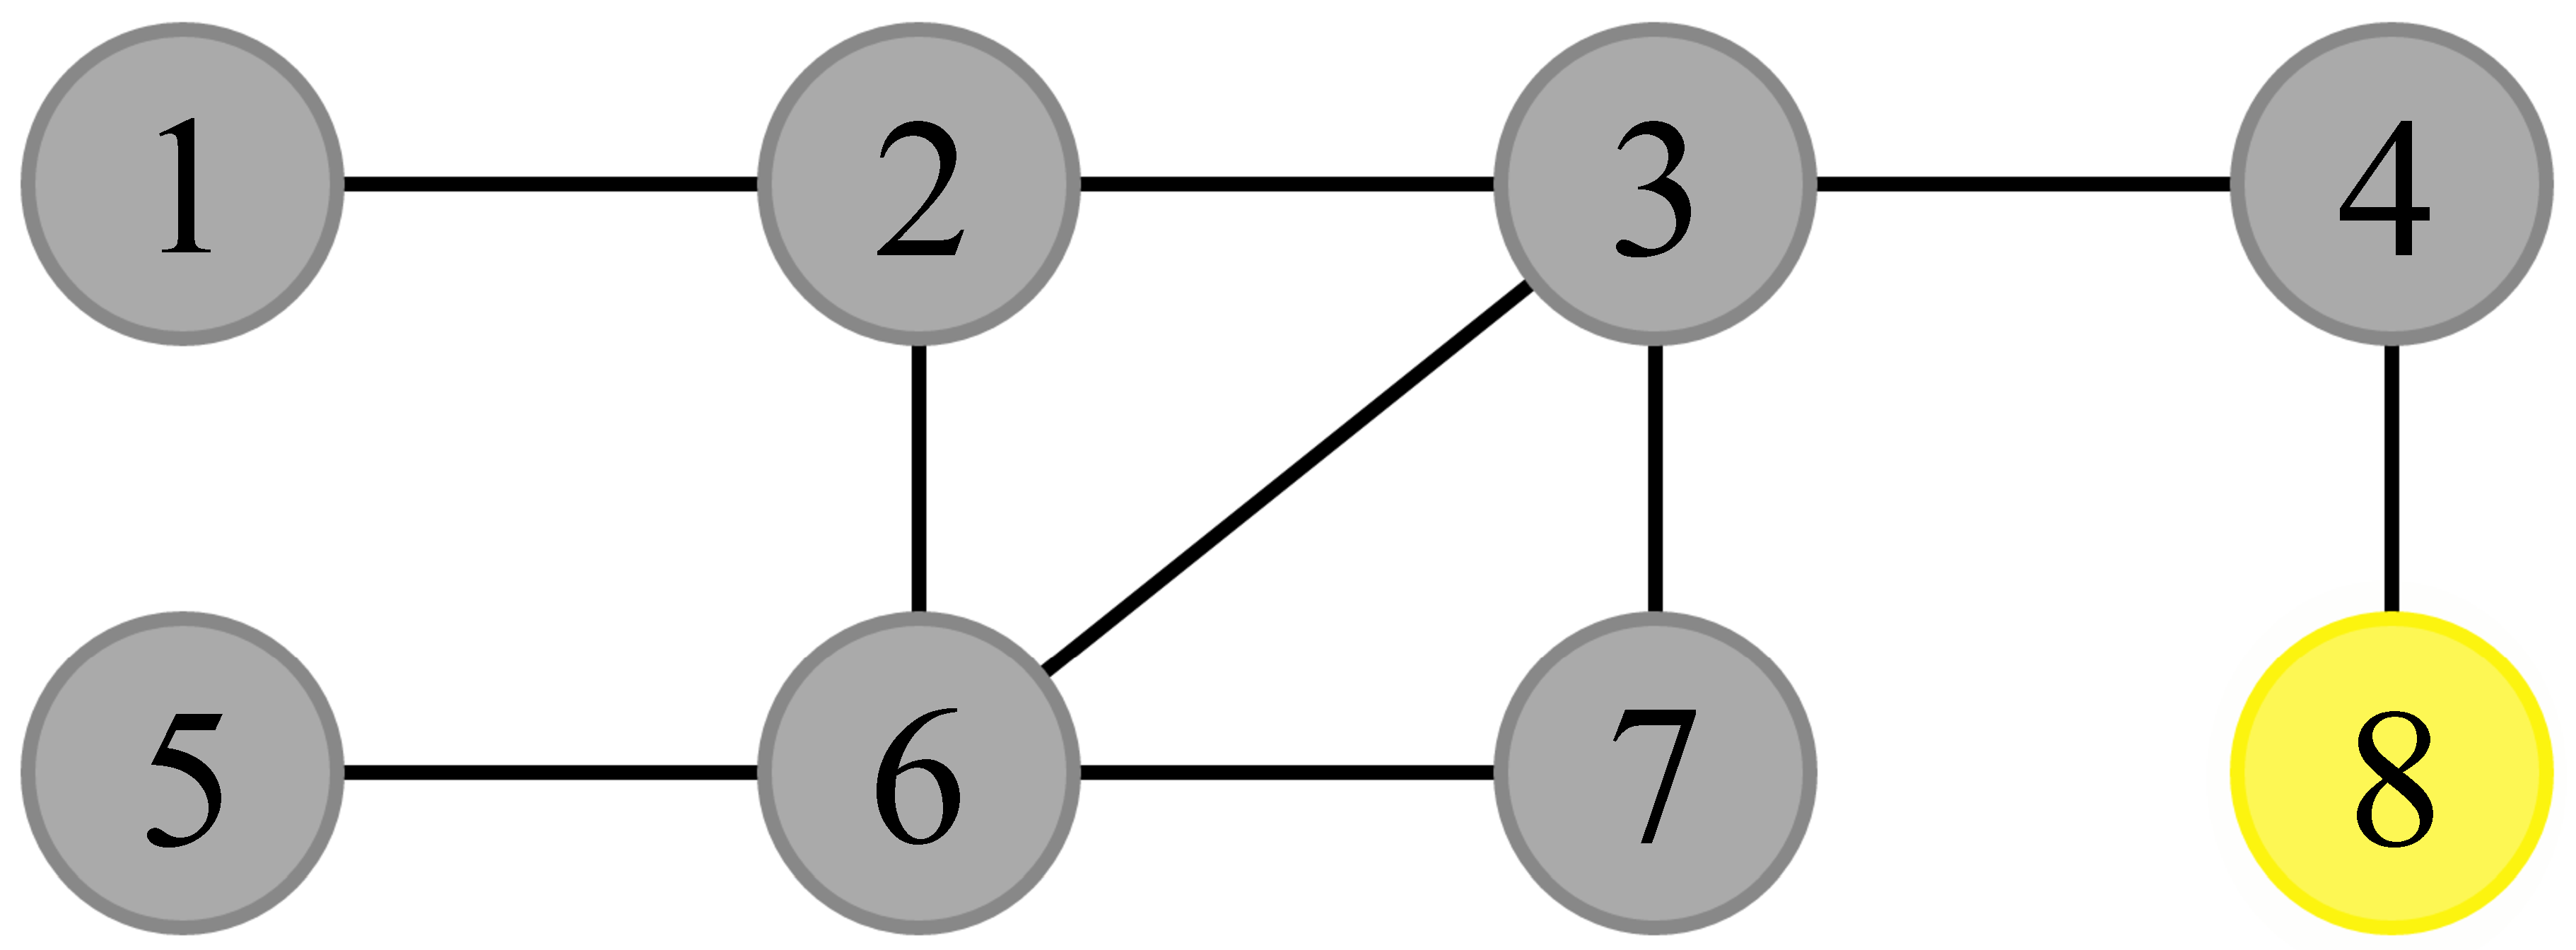
\includegraphics[width=6cm]{../figures/algorithm1-slide-1.pdf}
                \caption*{A simple, undirected graph $G$}
              \end{figure}
            \end{textblock*}
          \end{center}
        \end{column}
      \end{columns}
    }

  \end{frame}

  \section{CF Coloring for Planar Graphs}

  \begin{frame}[standout]
    \centering
    {Thanks to Peter Dolan, Elena Machkasova,

    and Peh Ng for their advice and feedback.}
    \vfill
    \href{https://github.com/devshawn/senior-seminar}{github.com/devshawn/senior-seminar}
    \vfill
    \ccbyncsa{}
  \end{frame}

\end{document}
